\documentclass[11pt, a4paper, oneside, UTF8]{ctexbook}
\usepackage{amsmath, amsthm, amssymb, bm, graphicx, hyperref, mathrsfs, enumitem, geometry, listings, xcolor, listings, fontspec, caption}

% 标题、作者、创建日期
\title{{\Huge{\textbf{PL/SQL学校课程笔记}}}\\ORACLE}
\author{徐鸣飞}
\date{2023年12月27日}

% 设置全局字体
\setmainfont{Times New Roman}   %设置英文正常字体为Times New Roman
\let\kaishu\relax %清除旧定义
\newCJKfontfamily\kaishu{KaiTi}[AutoFakeBold] %重定义\kaishu

% 设置页面的尺寸和布局。
\geometry{a4paper,scale=0.75}

% 行间距为1.5倍
\linespread{1.5}

% 定义定理环境
\newtheorem{theorem}{定理}[chapter]
\newtheorem{definition}[theorem]{定义}
\newtheorem{lemma}[theorem]{引理}
\newtheorem{corollary}[theorem]{推论}
\newtheorem{example}[theorem]{例}
\newtheorem{proposition}[theorem]{命题}

% 自定义配置
% 设置全局的 enumerate 环境项之间的距离
\setlist[enumerate]{itemsep=5pt, parsep=0pt, leftmargin=20pt, topsep=5pt, partopsep=0pt}
\setlist[itemize]{itemsep=5pt, parsep=0pt, leftmargin=20pt, topsep=5pt, partopsep=0pt}
% 定义新环境
% 定义颜色
\definecolor{commentcolor}{RGB}{182,73,1}
% 定义代码
\lstnewenvironment{java}[1][]{
  \lstset{
    language=Java,
    basicstyle=\ttfamily,
    keywordstyle=\color{blue},
    commentstyle=\color{green!60!black},
    stringstyle=\color{commentcolor},
    showstringspaces=false,
    breaklines=true,
    frame=single,
    flexiblecolumns=true,
    backgroundcolor=\color{gray!5},
    numbers=left,
    numberstyle=\tiny,
    #1
  }
}{}
\lstnewenvironment{plsql}[1][]{
  \lstset{
    language=SQL,
    morekeywords={BEGIN,DECLARE,END,IF,ELSE,ELSIF,LOOP,WHILE,PROCEDURE,FUNCTION},
    basicstyle=\ttfamily,
    keywordstyle=\color{blue},
    commentstyle=\color{green!60!black},
    stringstyle=\color{commentcolor},
    showstringspaces=false,
    breaklines=true,
    frame=single,
    flexiblecolumns=true,
    backgroundcolor=\color{gray!5},
    numbers=left,
    numberstyle=\tiny,
    #1
  }
}{}

% 文章开始
\begin{document}

% 生成标题
\maketitle

% 生成目录
\newpage                    %新的一页
\pagenumbering{Roman}       %页码以大写罗马数字形式表示
\setcounter{page}{1}        %设置当前页为第一页
\tableofcontents            %生成目录

% 生成内容
\newpage                    %新的一页
\pagenumbering{arabic}      %页码以阿拉伯数字形式表示
\setcounter{page}{1}        %设置当前页为第一页

% 文章内容
\chapter{导言}
\section{常见数据库}
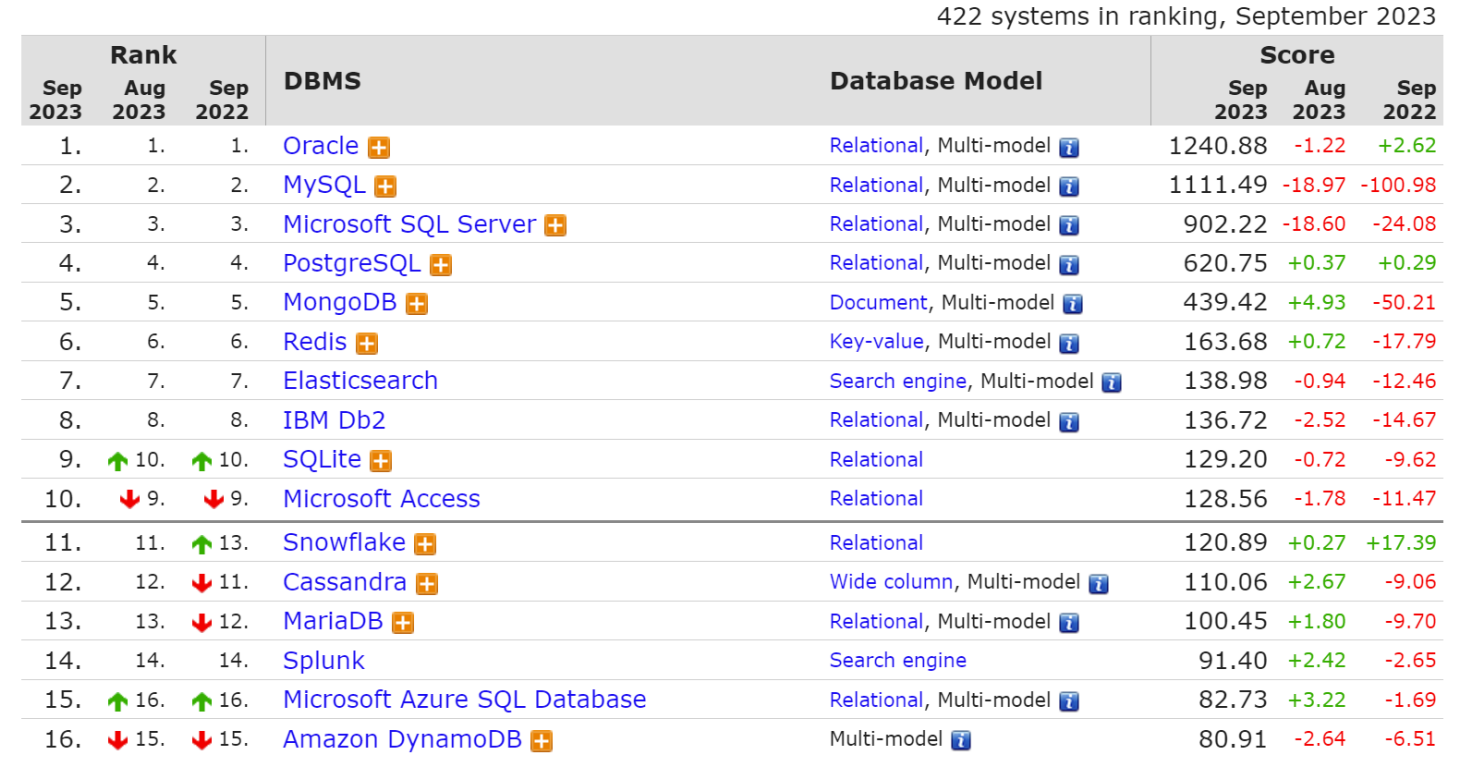
\includegraphics[width=0.9\linewidth]{picture/数据库占比对比.png}
\subsection{关系型数据库}
\subsubsection{MySQL}
MySQL是一款\textbf{开源的关系型数据库管理系统(RDBMS)},由瑞典MySQL AB公司开发,现由Oracle公司维护。以其轻量级、高效、快速的特性而闻名,适用于中小型应用和网站。MySQL支持多平台运行,包括Windows、Linux、macOS等,提供多种存储引擎如InnoDB、MyISAM等,具备良好的扩展性和广泛的社区支持。作为开源软件,MySQL允许用户免费获取、使用和修改其源代码,成为广泛应用于Web开发和其他应用场景的可靠数据库解决方案。
\subsubsection{Oracle}
Oracle是一款\textbf{商业性质的关系型数据库管理系统(RDBMS)},由Oracle公司开发。以其丰富的功能集、高级事务管理、安全性和卓越的性能而著称,适用于大型企业级应用。Oracle数据库支持复杂查询、分布式数据库、以及高并发环境下的大规模数据处理,具备出色的可伸缩性和性能优化特性。作为商业软件,Oracle提供了专业的技术支持、认证体系和咨询服务,成为众多大型组织和企业信赖的数据库解决方案。
\subsection{NoSQL数据库}
\subsubsection{文档型数据库:MongoDB}
\textbf{MongoDB是一种非关系型数据库管理系统(NoSQL DBMS),以其面向文档的存储模型而著称。}由MongoDB公司开发,采用分布式架构和灵活的模式设计,适用于处理大量非结构化或半结构化的数据。MongoDB的数据存储形式为BSON(Binary JSON),支持动态模式,使得数据存储和查询更加灵活。其强大的横向扩展性和自动分片功能使得MongoDB适用于大规模数据存储和处理,尤其在Web应用、大数据和实时分析等场景中表现出色。由于其开源特性,MongoDB拥有庞大的社区支持,为开发人员提供了丰富的资源和工具。
\subsubsection{搜索引擎:Elasticsearch}
\textbf{Elasticsearch是一种分布式数据库管理系统,专注于搜索和分析大规模数据。}作为开源软件,Elasticsearch构建在Apache Lucene之上,采用文档导向的存储模型,以JSON格式存储数据。其核心能力包括实时搜索、结构化查询和复杂分析,使其成为处理实时数据和日志、构建全文搜索引擎以及进行大规模数据分析的理想选择。通过支持分布式架构,Elasticsearch实现了水平扩展,能够应对高负载和大规模数据存储需求。该系统与Kibana等工具的整合形成了ELK堆栈,为用户提供了全面的数据管理、搜索和可视化解决方案。
\subsubsection{key-value数据库:redis}
\textbf{Redis是一款开源、高性能的键值对存储系统,属于NoSQL数据库的一种。}作为内存数据库,Redis将数据存储在内存中,提供了快速的读写访问速度,适用于对性能有严格要求的场景。其特色包括支持多种数据结构(如字符串、哈希表、列表、集合等),原子性操作,发布订阅机制等。虽然主要用于缓存、会话管理和实时数据分析等领域,但由于其快速响应和可持久化存储的能力,也在一些应用中用作主数据库。Redis的灵活性、简单性和高可用性,使其成为各种实时应用和分布式系统的理想选择。
\section{数据库发展趋势}
\subsection{1960s-1980s:层次数据库}
20世纪60年代到80年代的数据库技术被称为“层次结构”,也可以被称为网状结
构,无论标签是什么,这个时代的想法都旨在以树状结构组织数据结构。

\textbf{换而言之,这个时代的数据库技术是将数据存储为相互链接的记录。}
\begin{figure}[htbp]
  \center
  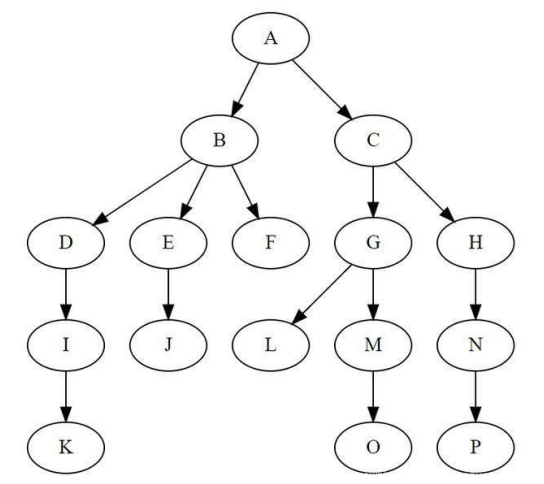
\includegraphics[width=0.5\textwidth]{picture/层次数据库示意图.png}
  \caption{层次数据库示意图}
  \label{fig:hierarchicalDatabase}
\end{figure}
在层次数据库的模型中,数据以节点的形式存在,每个节点可以包含一个或多个字段,形成父子关系。根节点是顶层节点,而叶节点是没有子节点的底层节点。层次数据库适用于需要表示层次结构信息的场景,如组织结构、文件系统等。尽管在过去曾经流行,但由于关系型数据库的普及,层次数据库在现代数据库系统中的应用相对较少。其特点包括数据重复、路径的唯一性以及专门的查询语言用于数据检索和更新。
\subsection{1980s-2000s:实体关系数据库}
实体关系数据库(Entity-Relationship Database)是一种基于实体-关系模型的数据库系统,用于存储和管理数据。在这个模型中,数据以实体(Entity)和实体之间的关系(Relationship)为核心。每个实体都有属性,而实体之间的关系描述了这些实体之间的联系和交互。

实体关系数据库的优势在于其规范化的数据结构、ACID 特性(原子性、一致性、隔离性、持久性)以及使用 SQL(Structured Query Language)进行数据操作和查询的能力。这种数据库模型在处理复杂的关联数据和支持事务处理方面表现出色,因此在各种应用场景中广泛应用,包括企业应用、金融系统、医疗信息管理等。

关系型数据库采用了关系代数的概念,数据以表格(表)的形式组织,每个表表示一个实体,表中的行代表实体的具体实例,而列代表实体的属性。实体之间的关系则通过外键来建立。
\begin{figure}[htbp]
  \center
  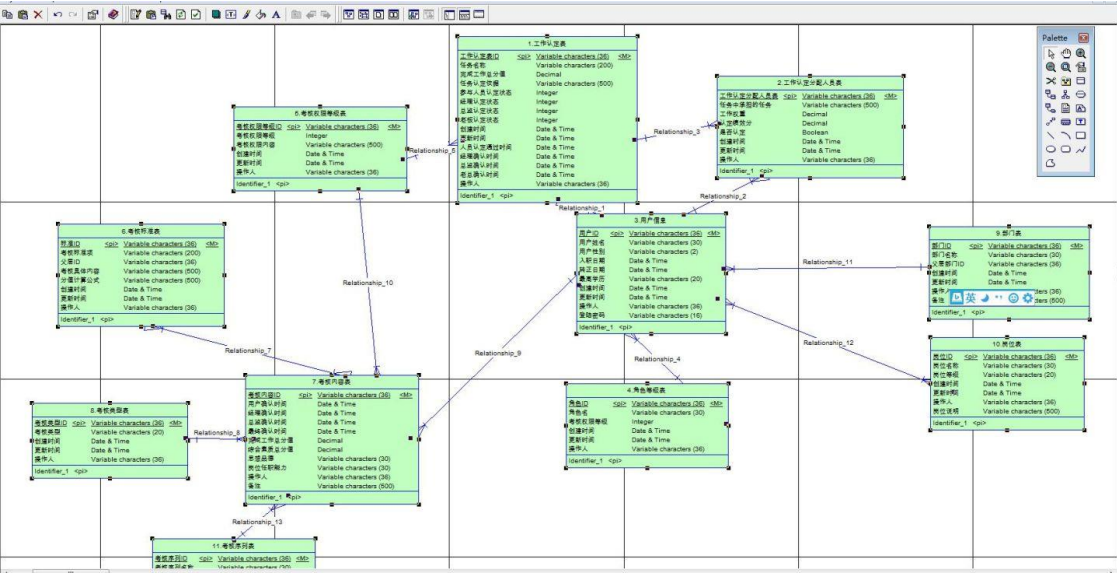
\includegraphics[width=0.5\textwidth]{picture/实体关系数据库示意图.png}
  \caption{实体关系数据库示意图}
  \label{fig:relationDatabase}
\end{figure}
\subsection{2000s-2020s:NoSQL}
NoSQL为Not Only SQL的缩写,是对不同于传统的关系型数据库的数据库管理系统的统称。

{\bfseries\kaishu 网络上的数据本质上不是表格的结构。}

NoSQL常用于超大规模数据的存储(例如谷歌或Facebook每天为他们的用户收集万亿比特的数据)。这些类型的数据存储不需要固定的模式,无需多余操作就可以横向扩展。

\begin{center}
  \begin{minipage}{\textwidth}
    \center
    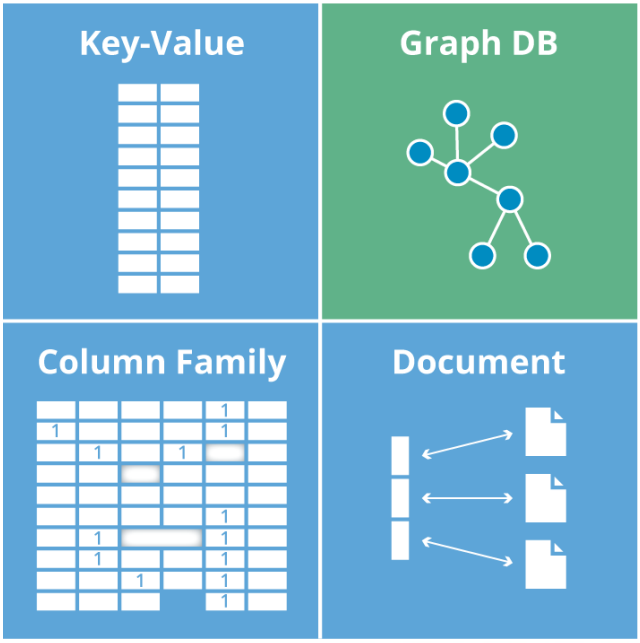
\includegraphics[width=0.5\textwidth]{picture/NoSQL数据库示意图.png}
    \captionsetup{hypcap=false}
    \captionof{figure}{NoSQL数据库示意图}
    \label{fig:NosqlDatabase}
  \end{minipage}
\end{center}

\subsection{2020s-未知:图数据库}
这个创新时代正在从存储系统的效率转向\textbf{从存储系统包含的数据中提取价值}。

\textit{即价值从效率转移到高度连接的数据资产中衍生。}

\section{SQL*Plus工具}
\subsection{介绍}
SQLPlus是Oracle数据库系统中的一种交互式查询工具和脚本处理器。它是一个{\bfseries\kaishu 命令行工具},允许用户连接到Oracle数据库并执行SQL查询、PL/SQL块以及其他数据库管理任务。

\subsection{交互过程}
\begin{center}
  \begin{minipage}{\textwidth}
    \center
    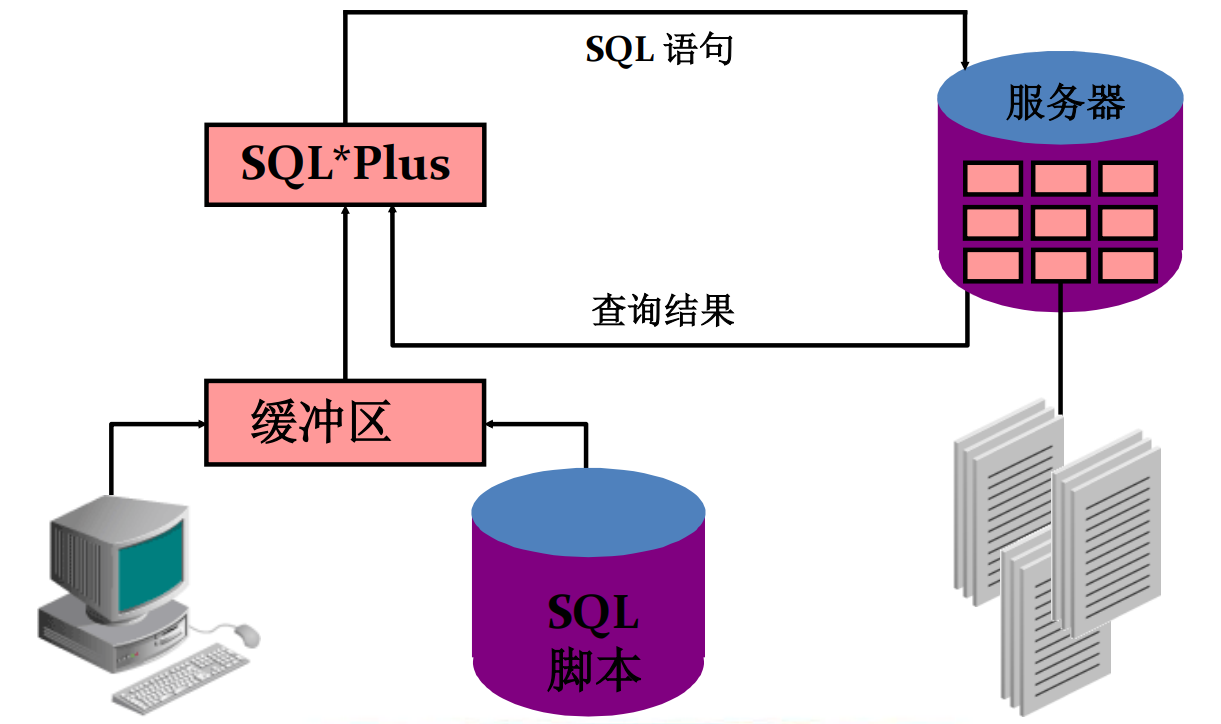
\includegraphics[width=0.7\textwidth]{picture/SQLPLUS交互.png}
    \captionsetup{hypcap=false}
    \captionof{figure}{SQL*Plus交互示意图}
    \label{fig:SQLPLUS交互}
  \end{minipage}
\end{center}
参与组件介绍:
\begin{description}
  \item[用户界面] 用户与SQLPlus进行交互的地方,可以是命令行界面或其他支持SQLPlus的用户界面。用户通过这个界面输入SQL查询、PL/SQL块或SQL*Plus命令。
  \item[SQL*Plus引擎] SQLPlus引擎是一个解释器,负责解释和执行用户输入的SQLPlus命令,以及管理与Oracle数据库的交互。它解析并执行SQL查询、PL/SQL块,处理输出格式,管理连接和会话等。
  \item[OCI(Oracle Call Interface)] OCI是Oracle数据库提供的一组API(应用程序接口),允许应用程序(包括SQLPlus)与Oracle数据库进行通信。\textbf{SQLPlus使用OCI}与数据库建立连接、发送SQL命令,以及接收执行结果。
  \item[Oracle数据库引擎] 这是实际执行SQL查询、PL/SQL块的地方。当SQLPlus将命令发送给数据库时,Oracle数据库引擎负责解析和执行这些命令,然后返回结果给SQLPlus。
  \item[数据缓冲区] SQL*Plus通常会在本地维护一个数据缓冲区,用于存储从数据库检索到的数据。这使得用户可以在本地对结果进行分析、浏览和编辑。
  \item[命令缓冲区] 用于存储执行过的SQL语句或PL/SQL块,以便可以轻松地重新执行它们或进行修改。当在SQL*Plus中输入一个SQL语句或PL/SQL块并按下Enter键时,该语句会被存储在命令缓冲区中,以便稍后再次使用。
\end{description}
\subsection{Oracle数据库连接命令}
在CMD中运行SQLPlus并连接到Oracle服务器的命令为:

{\bfseries\kaishu sqlplus <用户名>/<密码>@//<数据库IP>:<Port>/<服务名>}

如:
\begin{example}
  sqlplus system/system@//192.168.146.132:1521/helowin
\end{example}

\subsection{常用编辑命令}
\begin{description}
  \item[DESC] DESCRIBE,显示表结构,包括表的列名、数据类型和约束信息,效果见图\ref{fig:DESC_SQLPLUS}。
  \item[L] 列出当前缓冲区中的 SQL 语句(未执行)的命令。
    \item[\textup{[N]}] number,选中第n行;[n]后可追加内容[text]来替换第n行或新建第n行。
  \item[A] APPEND,追加文本到缓冲区中的当前选中行。使用“.”单独一行表示结束追加。使用前要求缓冲区内存在文本。
  \item[C] CHANGE,修改缓冲区中的当前选中行的文本,格式为{\bfseries\kaishu C /<原文>/<新文>}。
  \item[DEL] DELETE,删除缓冲区中的当前选中行。可追加[n]代表删除第n行;追加[n][m]删除第n至m行。
  \item[$\boldsymbol{/}$] 运行在SQL缓冲区中的SQL语句。
  \item[CL] CLEAR,清除 SQL*Plus 屏幕上的内容,将屏幕滚动条移至顶部。
\end{description}
\begin{figure}[htbp]
  \center
  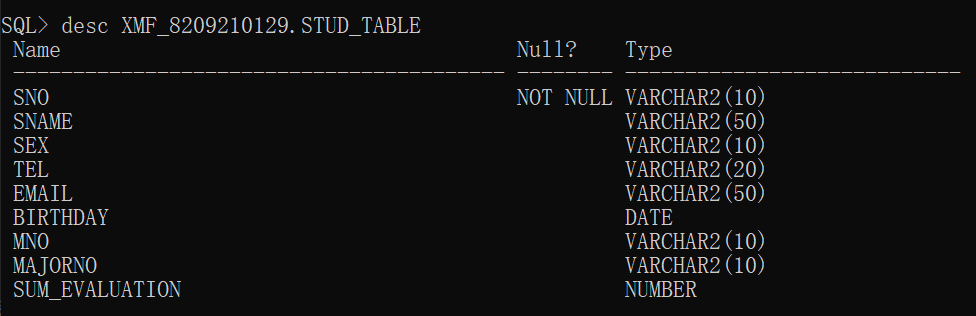
\includegraphics[width=\textwidth]{picture/DESC_SQLPLUS效果.png}
  \caption{DESC效果图}
  \label{fig:DESC_SQLPLUS}
\end{figure}

使用编辑缓冲区的命令前,需保证缓存区中存在内容:

\begin{center}
  \begin{minipage}{\textwidth}
    \center
    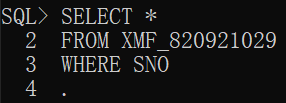
\includegraphics[width=0.5\textwidth]{picture/输入内容到缓冲区.png}
    \captionsetup{hypcap=false}
    \captionof{figure}{输入内容到缓冲区,使用enter换行,使用单独的.结束}
    \label{fig:输入内容到缓冲区}
  \end{minipage}
\end{center}

可使用L查看缓冲区:

\begin{center}
  \begin{minipage}{\textwidth}
    \center
    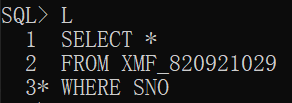
\includegraphics[width=0.5\textwidth]{picture/L命令效果.png}
    \captionsetup{hypcap=false}
    \captionof{figure}{L命令效果图}
    \label{fig:L命令效果}
  \end{minipage}
\end{center}

*号所在行为正在编辑行。
可使用数字更改选中行后,使用A命令添加内容:

\begin{center}
  \begin{minipage}{\textwidth}
    \center
    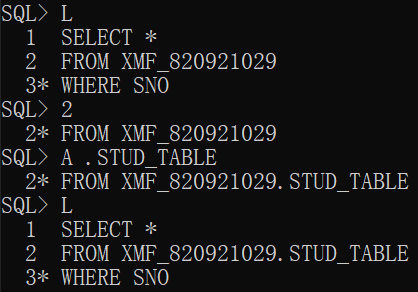
\includegraphics[width=0.5\textwidth]{picture/A命令效果.png}
    \captionsetup{hypcap=false}
    \captionof{figure}{A命令、n命令效果图}
    \label{fig:A命令效果}
  \end{minipage}
\end{center}

可使用C命令更改指定行(注意原文与新文中间无空格作为间隔):

\begin{center}
  \begin{minipage}{\textwidth}
    \center
    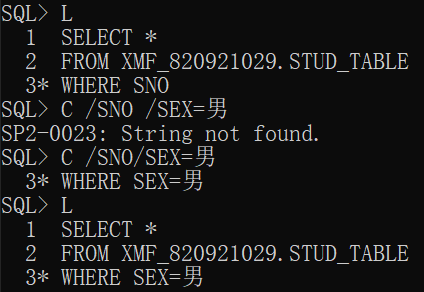
\includegraphics[width=0.5\textwidth]{picture/C命令效果.png}
    \captionsetup{hypcap=false}
    \captionof{figure}{C命令效果图}
    \label{fig:C命令效果}
  \end{minipage}
\end{center}

可使用DEL命令删除指定行:

\begin{center}
  \begin{minipage}{\textwidth}
    \center
    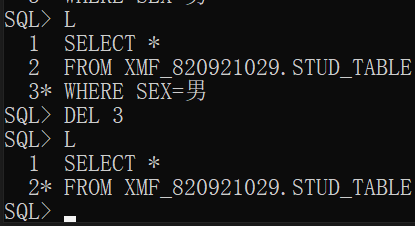
\includegraphics[width=0.5\textwidth]{picture/DEL命令效果.png}
    \captionsetup{hypcap=false}
    \captionof{figure}{DEL命令效果图}
    \label{fig:DEL命令效果}
  \end{minipage}
\end{center}

再次使用n命令新建行:

\begin{center}
  \begin{minipage}{\textwidth}
    \center
    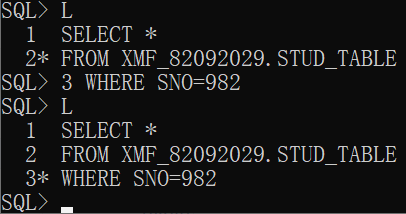
\includegraphics[width=0.5\textwidth]{picture/N命令效果图.png}
    \captionsetup{hypcap=false}
    \captionof{figure}{N命令效果图}
    \label{fig:N命令效果}
  \end{minipage}
\end{center}

使用$\boldsymbol{/}$运行(使用后缓冲区不会被清除):

\begin{center}
  \begin{minipage}{\textwidth}
    \center
    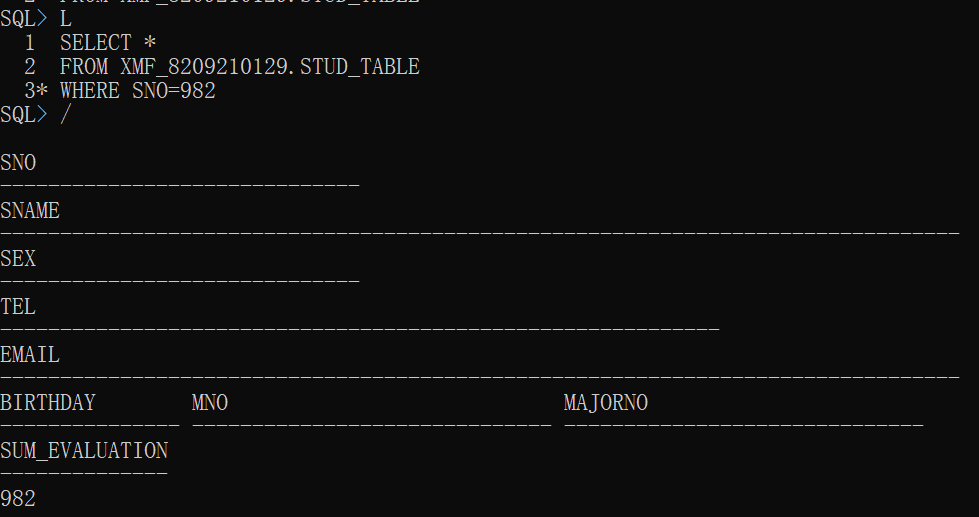
\includegraphics[width=0.5\textwidth]{picture/运行命令效果图.png}
    \captionsetup{hypcap=false}
    \captionof{figure}{运行命令效果图}
    \label{fig:运行命令效果}
  \end{minipage}
\end{center}

\subsection{SQL文件存取命令}

\begin{description}
  \item[SAVE] 把SQL缓冲区的内容存入指定的文件,如 \textit{SAVE D:\textbackslash SQL\textbackslash SMAPLE}。
  \item[GET] 将指定的脚本文件装入SQL缓存区,如\textit{GET D:\textbackslash SQL\textbackslash SMAPLE}。
  \item[START] @ 或START,把指定的脚本文件装入SQL缓冲区并运行,如\textit{@ D:\textbackslash SQL\textbackslash SMAPLE.sql}。
\end{description}

\subsection{输出保存命令}
SPOOL 命令用于将输出结果保存到文件中。该命令可以将 SQL 查询结果、PL/SQL 块的输出等保存到一个文件,这对于记录和分析数据库操作非常有用。
语法为:\\
{\bfseries\kaishu SPO[OL] [File\_name[.ext]] [[CRE[ATE]|REP[LACE]|APP[END]] | OFF | OUT ]}。

参数说明:
\begin{description}
  \item[File\_name] 指定脱机文件的名称,默认的文件扩展名为LST。
    \item[\textup{CRE[ATE]}] 表示创建一个新的脱机文件,这也是SPOOL命令的默认状态。
    \item[\textup{REP[LACE]}] 表示替代已经存在的脱机文件。
    \item[\textup{APP[END]}] 表示把脱机内容附加到一个已经存在的脱机文件中。
  \item[OFF | OUT] 表示关闭SPOOL输出。
\end{description}

% \chapter{PL/SQL语法学习}
\chapter{PL/SQL概述}
\section{介绍}
\textbf{PL/SQL(Procedural Language/Structured Query Language)}:一种\textbf{过程化编程语言},专门用于\textbf{Oracle数据库系统}。它将SQL(Structured Query Language)语句与结构化程序设计语言(如条件、循环等)相结合,提供了一种强大的方式来处理和操作数据库中的数据。

\section{优点}
\begin{enumerate}
  \item {\bfseries\kaishu 数据库集成:} PL/SQL是为数据库设计的,能够直接嵌套在SQL中;许多与数据库有关的应用程序功能都已经集成在PL/SQL语言中。
  \item {\bfseries\kaishu 模块化开发:} PL/SQL允许将代码模块化组织,通过存储过程和包的方式来管理和封装代码。这有助于提高代码的可维护性和重用性。
  \item {\bfseries\kaishu 性能优化:}PL/SQL支持存储过程和函数,可以在数据库中预编译和存储,提高了执行效率。此外,PL/SQL还支持游标,能够有效地处理大量的数据。
\end{enumerate}
此外,还有其他如\textbf{安全性}(PL/SQL能够帮助限制对数据库的直接访问,从而提高了数据库的安全性)、\textbf{灵活性}(PL/SQL具有丰富的控制结构和数据类型,使其既可以用于简单的SQL查询,也可以用于复杂的业务逻辑实现)、\textbf{事务控制}( PL/SQL提供了强大的事务控制功能,支持原子性、一致性、隔离性和持久性(ACID属性))等优点。

\section{执行体系}
\begin{center}
  \begin{minipage}{\textwidth}
    \center
    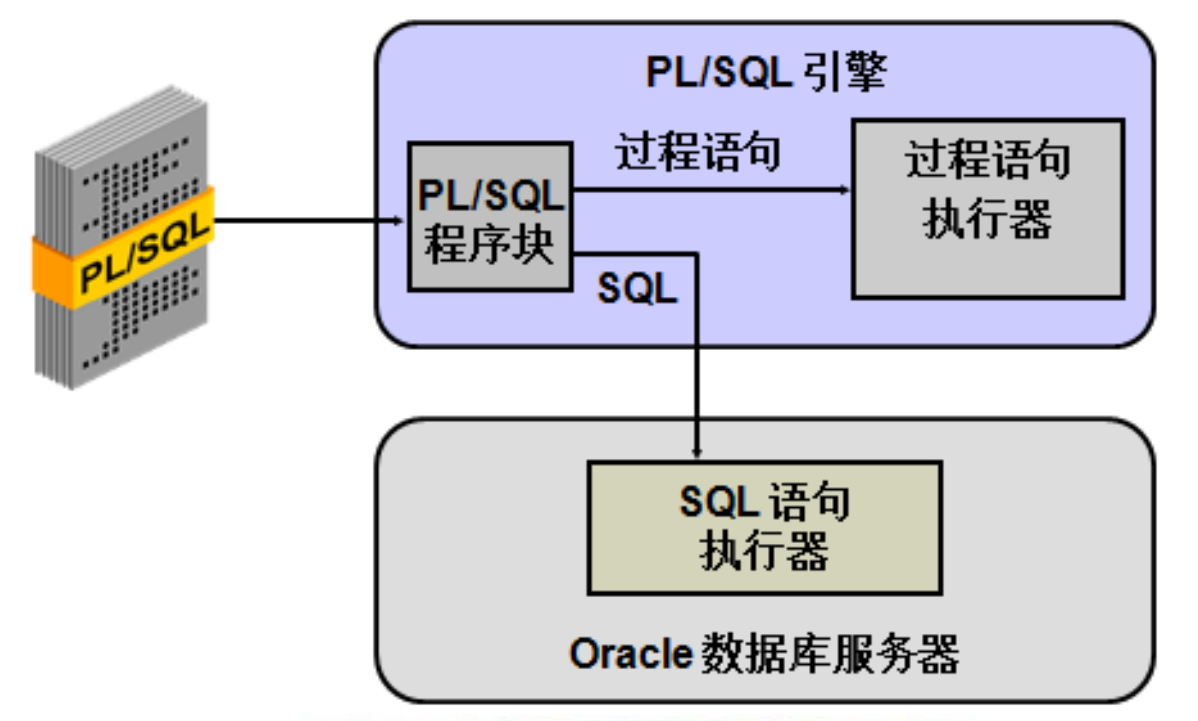
\includegraphics[width=0.5\textwidth]{picture/PLSQL执行体系.png}
    \captionsetup{hypcap=false}
    \captionof{figure}{PLSQL执行体系示意图}
    \label{fig:PLSQL执行体系}
  \end{minipage}
\end{center}
从图\ref{fig:PLSQL执行体系}中这些组件的角度来看PL/SQL的执行过程:
\begin{description}
  \item[PL/SQL引擎] \hfill
    \begin{itemize}
      \item PL/SQL解释器: 编译后的PL/SQL代码由PL/SQL引擎的解释器执行。解释器负责逐行执行PL/SQL代码,并管理变量、控制流程、处理异常等。
      \item 数据交互: 在PL/SQL执行过程中,可能涉及到与数据库的交互,例如执行SQL语句、操作数据等。这些交互通过PL/SQL引擎协调实现。
    \end{itemize}
  \item[过程语句执行器] \hfill
    \begin{itemize}
      \item 编译过程性代码: 过程语句执行器会编译PL/SQL代码,将其转换为可执行的形式。这个编译过程包括语法检查、编译成中间代码等步骤。
      \item 过程语句解析: 如果PL/SQL程序包含了过程性语句,这些语句将被PL/SQL引擎的过程语句执行器处理。这可能包括存储过程、函数或触发器的调用。
    \end{itemize}
  \item[SQL执行器]  \hfill
    \begin{itemize}
      \item 接收SQL语句: 当一个包含PL/SQL代码的程序被触发时,其中可能包含SQL语句。这些SQL语句被传递给SQL执行器,它负责执行这些语句。
      \item 解析SQL语句: SQL执行器解析SQL语句,进行语法分析和语义检查。在这个阶段,执行计划被生成,这是一个描述如何执行查询的内部表示。
    \end{itemize}
  \item[Oracle数据库服务器] \hfill
    \begin{itemize}
      \item 数据存储和检索: 当PL/SQL程序执行SQL语句时,Oracle数据库服务器负责实际的数据存储和检索。执行计划告诉数据库服务器如何最有效地执行查询,并从表中检索或修改数据。
    \end{itemize}
\end{description}

当有过程调用或SQL语句执行时,流程可能涉及多次从PL/SQL引擎到SQL执行器,再到数据库服务器的交互。

需要注意的是,Oracle数据库的内部执行细节是复杂的,并且可能受到优化、缓存、并发控制等多方面的影响。

\chapter{程序块结构}
\section{程序块}
PL/SQL程序块是PL/SQL语言中的基本结构,它可以包含变量、常量、游标、异常处理等元素。PL/SQL程序块有三种主要形式:{\bfseries\kaishu 匿名块、存储过程和存储函数。}

\begin{enumerate}
  \item {\bfseries\kaishu 匿名块(Anonymous blocks)}:没有命名的程序块。匿名块是在应用程序内部需要的地方声明的,在这个应用程序每次执行时,这些匿名块都会被编译并执行。
  \item  {\bfseries\kaishu 过程(Procedures)}和{\bfseries\kaishu 函数 (Functions) }:过程和函数也统称为{\bfseries\kaishu 子程序 (Subprograms)},子程序是对匿名块的补充,子程序就是被命名的PL/SQL程序块,而它们可以存储在数据库中。
\end{enumerate}
一个简单的PL/SQL匿名块的结构如下:
\begin{plsql}[caption=PL/SQL匿名块示例代码]
DECLARE
  -- 声明变量和常量
  variable_name datatype;
  constant_name CONSTANT datatype := value;

BEGIN
  -- 可执行的PL/SQL代码
  -- 可以包括各种语句,如赋值、条件语句、循环等
  -- 例如:
  variable_name := value;
  IF condition THEN
  -- do something
  END IF;

EXCEPTION
  -- 异常处理部分
  -- 处理可能出现的异常
  -- 例如:
  WHEN others THEN
  -- handle exception

END;
/
\end{plsql}
一个简单的PL/SQL函数的示例代码(获取员工薪水):
\begin{plsql}[caption=获取员工薪水函数示例代码]
CREATE OR REPLACE FUNCTION get_employee_salary(p_employee_id NUMBER)
  RETURN NUMBER
  IS
  -- 声明变量
  v_salary NUMBER;
BEGIN
  -- 查询员工薪水
  SELECT salary INTO v_salary
  FROM employees
  WHERE employee_id = p_employee_id;

  -- 返回薪水
  RETURN v_salary;
END;
/
\end{plsql}
一个简单的PL/SQL过程的示例代码(更新员工薪水):
\begin{plsql}[caption=更新员工薪水过程示例代码]
CREATE OR REPLACE PROCEDURE update_employee_salary(p_employee_id NUMBER, p_new_salary NUMBER)
  IS
BEGIN
  -- 更新员工薪水
  UPDATE employees
  SET salary = p_new_salary
  WHERE employee_id = p_employee_id;

  -- 提交事务
  COMMIT;
END;
/
\end{plsql}
程序块结构说明:
\begin{description}
  \item[DECLARE] {\bfseries\kaishu 可选},\textit{声明段},以关键字DECLARE开始并以执行段的开始而结束。
  \item[BEGIN] {\bfseries\kaishu 必选},\textit{执行段},以关键字BEGIN开始而以关键字END或关键字EXCEPTION结束。
  \item[EXCEPTION] {\bfseries\kaishu 可选},\textit{异常处理段},以关键字EXCEPTION开始,以关键字END结束。
\end{description}
执行规则:
\begin{enumerate}
  \item 每一个PL/SQL控制语句都是以分号(;)结束。
  \item 使用正斜杠(/)运行SQL*Plus内存缓冲区的匿名PL/SQL程序块。
\end{enumerate}

\section{程序块的嵌套}
因为PL/SQL是一个过程化的程序设计语言,所以它具备语句嵌套能力。只要运行执行语句存在的地方就可以使用嵌套程序块,这种嵌套式可以许多层的。

在一个PL/SQL程序块中声明的变量(标识符)对于这一程序块本身来说是局部(本地)变量,而对于所有子块就是全局变量。如果一个全局变量在一个子块中又再次进行了声明(与全局变量同名),内部块中的变量将隐藏外部块中的同名变量。

\begin{plsql}[caption=程序块嵌套示例代码]
DECLARE
  -- 全局变量
  global_var NUMBER := 10;
BEGIN
  DBMS_OUTPUT.PUT_LINE('Global Variable: ' || global_var);
 
  -- 子块中声明同名的局部变量
  DECLARE
    local_var NUMBER := 20; -- 局部变量
  BEGIN
    DBMS_OUTPUT.PUT_LINE('Local Variable: ' || local_var);
    -- 在子块中使用局部变量,优先使用局部变量的值
    global_var := 30; -- 修改全局变量
    DBMS_OUTPUT.PUT_LINE('Global Variable (Modified in Subblock): ' || global_var);
  END;
 
  -- 子块结束后,回到全局作用域
  DBMS_OUTPUT.PUT_LINE('Global Variable (Back to Global Scope): ' || global_var);
END;
\end{plsql}

\begin{center}
  \begin{minipage}{\textwidth}
    \center
    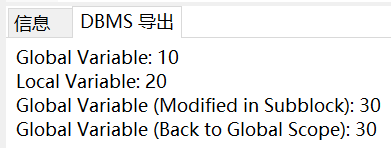
\includegraphics[width=0.5\textwidth]{picture/嵌套程序块示例代码运行结果.png}
    \captionsetup{hypcap=false}
    \captionof{figure}{嵌套程序块示例代码运行结果图}
    \label{fig:嵌套程序块示例代码运行结果}
  \end{minipage}
\end{center}


\chapter{变量}
 {\bfseries\kaishu 变量},就是内存中一个命名的临时存储区,而变量中所存储的信息就是这个变量的当前值。

在PL/SQL中,在使用一个变量之前,必须首先声明这个变量。一旦声明了这个变量,就可以在SQL语句和过程化(PL/SQL)语句中使用这个变量了。

变量使用步骤:
\begin{enumerate}
  \item 在声明部分(DECLARE块)\textbf{声明和初始化}变量
  \item 在执行部分(BEGIN块)为变量\textbf{赋新值}
  \item 通过参数将值传入PL/SQL块
  \item 通过输出变量来查看结构
\end{enumerate}
\section{变量命名规则}
\begin{itemize}
  \item 必须{\bfseries\kaishu 以英语字母开始}
  \item 可以包含{\bfseries\kaishu 英语字母}或{\bfseries\kaishu 数字}或{\bfseries\kaishu 特殊字符}——美元号(\$)、下划线(\_)、和井号(\#)
  \item 长度最长为{\bfseries\kaishu 30}个字符
  \item {\bfseries\kaishu 不区分大小写}
  \item 不能是保留关键字
  \item 不能(不宜)与数据库的表或列同名
\end{itemize}
\section{变量声明语法}
在引用PL/SQL程序块中的变量之前,必须在声明段声明所有的变量(标识符)。
在声明变量的同时还可以为变量赋初值,但是在声明变量时赋予初始值是可选的。
如果在一个变量声明中引用了其他变量,一定要确保在之前的语句中已经声明了引用的变量。

声明语法:
{\bfseries\kaishu 标识符 [CONSTANT] 数据类型 [NOT NULL] [<:= | DEFAULT> initial\_value]}

\begin{plsql}[caption=PL/SQL变量声明语法示例]
DECLARE
  v_dogid NUMBER(10) NOT NULL := 38;
  v_name VARCHAR2(25) := 'White Tiger'
  c_color CONSTANT VARCHAR2(15) := 'White'
  v_birthday DATE;
\end{plsql}

\section{变量数据类型}
PL/SQL支持四大类数据类型(最常用的是标量数据类型,目前熟悉这个即可):
\begin{enumerate}
  \item 标量(Scalar)数据类型:
        \begin{itemize}
          \item NUMBER: 用于存储数值,可以是整数或小数。
                \begin{itemize}
                  \item NUMBER(p,s):数据型数据,p 表示精度(总位数),s 表示小数部分的位数
                  \item BINARY\_INTEGER:基本整型数
                  \item PLS\_INTEGER:基本带符号整数型
                  \item BINARY\_FLOAT:存储单精度浮点数,以IEEE754格式表示浮点数,它需要5个字节来存储数字
                  \item BINARY\_DOUBLE:存储双精度浮点数,以IEEE754格式表示浮点数,它需要9个字节来存储数字
                \end{itemize}
          \item character: 字符型数据类型,用于存储字符串。
                \begin{itemize}
                  \item VARCHAR2(size):基本变长字符型数据
                  \item CHAR(size):基本定长字符型数据
                \end{itemize}
          \item DATE: 用于存储日期和时间。
                \begin{itemize}
                  \item DATA:基本日期和时间数据
                  \item TIMESATMP(precision):该数据类型除了日期和时间之外还包括了多达小数点后9位秒数
                \end{itemize}
          \item BOOLEAN: 用于存储布尔值(TRUE 或 FALSE)。
                \begin{itemize}
                  \item BOOLEAN:基本逻辑类型,它只能存储逻辑计算的3个可能值之一
                \end{itemize}
        \end{itemize}
  \item 组合(Composite)数据类型:
        \begin{itemize}
          \item \%ROWTYPE: 表示一个表行的结构,通常在变量声明中使用。
          \item RECORD: 类似于\%ROWTYPE,但可以自定义结构。
          \item TABLE: 用于存储同一数据类型的集合。可以是索引表(INDEX BY表,也称关联数组)或嵌套表。
        \end{itemize}
  \item 引用(Reference)数据类型:
        \begin{itemize}
          \item 游标(CURSOR):游标是一种引用数据类型,用于对查询结果进行迭代。可以使用显式游标或隐式游标。
          \item 引用游标(REF CURSOR): 用于存储游标引用,可用于动态查询结果的处理。
        \end{itemize}
  \item 大对象(LOB)数据类型:
        \begin{itemize}
          \item CLOB (Character Large Object): 用于存储大量字符数据,如文本。
          \item BLOB (Binary Large Object): 用于存储二进制数据,如图像、音频等。
          \item NCLOB (National Character Large Object): 类似于 CLOB,但用于存储国家字符集数据。
          \item BFILE: 用于存储二进制文件的地址引用,文件存储在数据库外部。
        \end{itemize}
\end{enumerate}
\section{变量命名建议}
\begin{enumerate}
  \item 遵守命名的规则,变量的命名规则与SQL对象的命名规则完全相同。
  \item 必须初始化被指定为非空(NOT NULL)和常量(Constant)的变量。
  \item 一行最好只声明一个标识符以提高代码的易读性和方便代码的维护。
  \item 通过使用赋值操作符(:=)或默认关键字(DEFAULT)来初始化标识符。
  \item 变量最好不要与列名重名。
  \item 两个PL/SQL变量(对象)只要在不同的程序块中是可以同名的。
  \item 如果没有必要就不要在PL/SQL变量上强加非空(NOT NULL)约束。
  \item 代码中使用了 PL/SQL 游标、BLOB/CLOB Locator 或其他需要手动释放的资源,请确保在不再需要它们时及时释放这些资源,以避免内存泄漏。
\end{enumerate}

\section{代替变量和绑定变量}
\subsection{代替变量}
因为PL/SQL本身没有输入和输出功能,所以必须依赖于执行PL/SQL程序的环境变量值传入或传出PL/SQL程序块。

在SQL*Plus环境中,可以使用{\bfseries\kaishu SQL*Plus的代替变量}将运行时的值传给PL/SQL程序块。在PL/SQL程序块中可以使用前导的\&符号引用代替变量,就像在SQL语句中引用SQL*Plus的代替变量一样。在PL/SQL程序执行前,正文的值被代替进PL/SQL程序块中。

例如,一个使用代替变量的查询可以如下所示:
\begin{plsql}[]
Select * 
FROM XMF_8209210129.STUD_TABLE 
WHERE SNO=&ReplaceVariable1;
\end{plsql}

运行效果:
\begin{center}
  \begin{minipage}{\textwidth}
    \center
    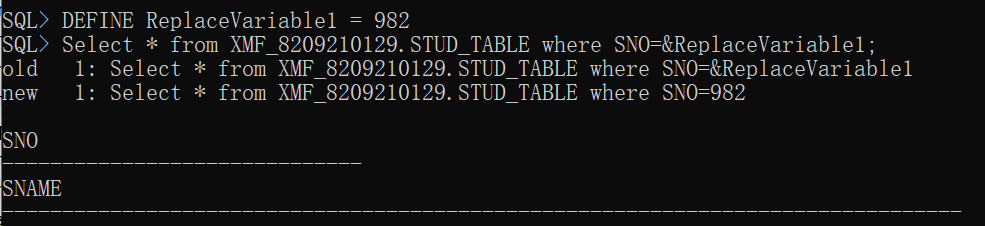
\includegraphics[width=\textwidth]{picture/代替变量案例.png}
    \captionsetup{hypcap=false}
    \captionof{figure}{代替变量案例运行结果}
    \label{fig:代替变量案例}
  \end{minipage}
\end{center}


在这里,ReplaceVariable1是一个代替变量,SQL*Plus会在执行查询之前提示用户输入ReplaceVariable1的值(如果未定义变量),并将其替换到SQL语句中。DEFINE ReplaceVariable1 = 982 用于定义SQLPlus变量。

注意:如果需要`\&variable '这样的字符串,可以使用两个连续的 \& 来避免 SQL*Plus 将其解释为代替变量,如\textbf{`\&\&your\_value'}。
\subsection{绑定变量}
绑定变量是在{\bfseries\kaishu 使用(或调用)PL/SQL的 环境}中创建的,而不是在PL/SQL程序的声明段中定义的。在一个PL/SQL程序块中声明的所有变量只在执行这个程序块时可以使用。而在这个程序块执行后,这些变量所使用的内存就释放了。然而,绑定变量则不同,在程序块执行后,绑定变量依然存在并允许访问。

绑定变量是在SQL语句中使用占位符(通常是冒号:后跟变量名)来代替实际的数值或表达式。{\bfseries\kaishu 在PL/SQL中,通过使用绑定变量,可以减少SQL语句的解析次数,提高性能。}绑定变量在SQL语句执行时被动态绑定,而不是在每次执行时重新解析整个SQL语句。

运行演示:
\begin{center}
  \begin{minipage}{\textwidth}
    \center
    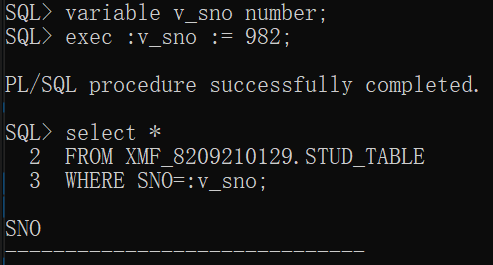
\includegraphics[width=0.5\textwidth]{picture/绑定变量效果.png}
    \captionsetup{hypcap=false}
    \captionof{figure}{绑定变量使用案例}
    \label{fig:绑定变量效果}
  \end{minipage}
\end{center}
\begin{description}
  \item[variable v\_sno number;] 定义绑定变量v\_sno
  \item[exec :v\_sno := 982] 给绑定变量赋值为982
\end{description}

\subsection{不同}

\begin{enumerate}
  \item {\bfseries\kaishu 绑定变量(Bind Variables)}
  \begin{itemize}
    \item 绑定变量是用于在SQL语句中传递数值或数据的一种机制,通过绑定变量,可以\textbf{将变量的值绑定到SQL语句中},而不是直接在SQL语句中使用硬编码的值。
    \item 这有助于提高性能,因为数据库可以缓存已编译的SQL语句,并在执行时仅替换绑定变量的值,而\textbf{不需要重新编译}整个SQL语句。
  \end{itemize}
  \item {\bfseries\kaishu 代替变量(Substitution Variables)}
  \begin{itemize}
    \item 代替变量是一种SQLPlus工具的功能,它允许在SQLPlus中使用变量,这些变量在脚本运行之前由用户手动输入,或者可以通过DEFINE命令定义。
    \item 代替变量在SQL*Plus脚本中被替换为相应的值,类似于\textbf{宏替换}。
  \end{itemize}
\end{enumerate}
\section{变量作用域}
一个变量(标识符)在声明它的程序块中是可见的,并且在所有嵌套的子块中也是可见的。如果一个PL/SQL块没有发现本地声明的变量,该PL/SQL程序块将向上查找包含它的父块,而不会向下查看所包含的子块或查找同一级别(没有嵌套关系)块。

作用域适用所有的对象,包括变量、游标、用户定义的异常和约束等。

\subsection{局部变量(Local Variables)}
\begin{enumerate}
  \item 局部变量是在一个程序块内部声明的变量,仅在该程序块内部可见和可访问。
  \item 局部变量的生命周期仅限于包含它的程序块的执行期间。\textbf{一旦程序块执行完毕,局部变量就会被销毁,不再可用。}
  \item 局部变量通常在DECLARE部分声明,并可以用于存储临时数据或中间计算结果。
\end{enumerate}

\begin{plsql}[caption=局部变量作用域示例]
DECLARE
  local_variable NUMBER := 10;
BEGIN
  -- 在此处访问和使用局部变量
END;
-- 局部变量在此处不可见
\end{plsql}

\subsection{嵌套局部变量(Nested Local Variables)}
\begin{enumerate}
  \item 嵌套程序块中声明的局部变量对外部程序块不可见,但对内部程序块可见。
  \item 如果内部程序块声明了与外部程序块相同名称的局部变量,它们不会相互冲突。{\bfseries\kaishu 内部变量会遮蔽外部变量。}
\end{enumerate}

\begin{plsql}[caption=嵌套局部变量作用域示例]
DECLARE
  outer_variable NUMBER := 10;
  PROCEDURE inner_procedure IS
    inner_variable NUMBER := 20;
  BEGIN
    -- 在内部程序块中,可以访问 inner_variable 和outer_variable
  END inner_procedure;
BEGIN
  -- 在外部程序块中,只能访问 outer_variable
END;
\end{plsql}

注意:此处定义了一个内部过程inner\_variable。

\subsection{全局变量(Global Variables)}
\begin{enumerate}
  \item 全局变量在整个PL/SQL块中声明,对所有程序块可见。
  \item 全局变量的生命周期与整个PL/SQL块的执行周期相同。
  \item 全局变量通常用于存储在多个程序块之间需要共享的数据。
\end{enumerate}

\section{布尔变量与布尔表达式}
布尔变量和布尔表达式在任何程序语言设计上都是非常重要和广泛使用的。在PL/SQL程序中,可以在SQL语句中也可以在过程化语句中进行变量的比较,这样的比较表达式被称为布尔表达式,它们是由单个表达式或由关系操作符所分隔的复杂表达式所组成。

特性:
\begin{itemize}
  \item 只有{\bfseries\kaishu 值TURE、FALSE和NULL}可以赋给一个布尔变量。
  \item 可以通过{\bfseries\kaishu 逻辑操作符AND、OR和NOT}对布尔变量进行运算,运算总是产生TURE、FALSE或NULL。
  \item 数字、字符和日期表达式可以被用来返回一个布尔值。
\end{itemize}
\subsection{布尔操作符(结果为布尔类型)}
\begin{center}
  \begin{minipage}{\textwidth}
    \center
    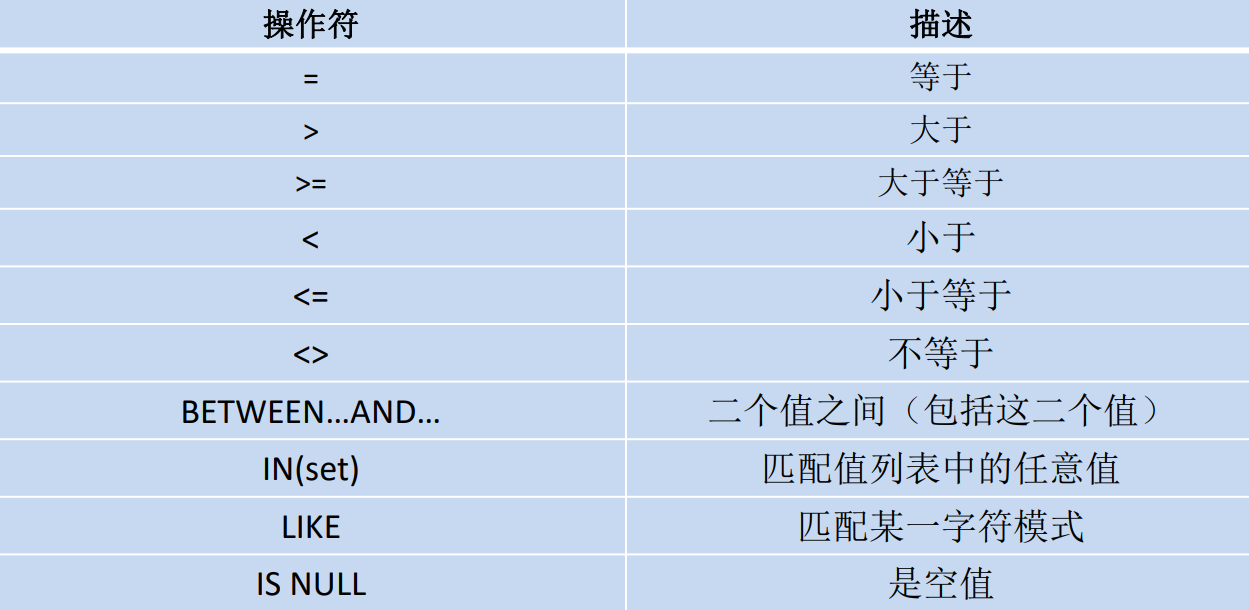
\includegraphics[width=\textwidth]{picture/布尔操作符.png}
    \captionsetup{hypcap=false}
    \captionof{figure}{布尔操作符}
    \label{fig:布尔操作符}
  \end{minipage}
\end{center}
\section{LOB变量}
大对象LOB是 large object的缩写,就意味着存储大量的数据,在数据库中,表中的列定义为LOB类型(如CLOB和BLOB)。利用LOB数据类型,可以在数据库中存储大量的无结构数据块(如正文、图形、声音和影像信息),其存储量可多达128T(数据量的多少取决于数据块大小)。
\subsection{LOB变量类型}
\subsubsection{CLOB数据类型(Character Large Object)}
CLOB用于在数据库中存储字节流类型的大数据对象,如演讲稿、说明书或简历等。
\subsubsection{BLOB数据类型(Binary Large Object)}
用于在数据库中存储大的二进制对象,如照片或幻灯片等。当从数据库中提取这样的数据或向数据库中插入这样的数据时,数据库并不解释这些数据。使用这些数据的外部应用程序必须自己解释这些数据。
\subsubsection{BFILE数据类型(Binary File)}
用于在数据库外的操作系统文件中存储大的二进制对象,如电影胶片等。与其他的LOB数据类型不同,BFILE数据类型是外部数据类型。BFILE类型是存储在数据库之外的,它们可能是操作系统文件。
\subsubsection{NCLOB数据类型(National Language Character Large Object)}用于在数据库中存储NCHAR类型的单字节或定长多字节的Unicode大数据对象。
\subsection{LOB变量使用}
\begin{plsql}[caption=LOB变量使用示例代码]
DECLARE
  clob_data CLOB;
  buffer VARCHAR2(32767);
  amount NUMBER;
  offset NUMBER := 1;
BEGIN
  -- 初始化 CLOB 数据
  clob_data := '这是一个CLOB示例。';
  -- 读取 CLOB 数据
  amount := DBMS_LOB.GETLENGTH(clob_data);
  DBMS_LOB.READ(clob_data, amount, offset, buffer);
  DBMS_OUTPUT.PUT_LINE(buffer);
END;
\end{plsql}

运行结果:
\begin{center}
  \begin{minipage}{\textwidth}
    \center
    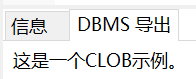
\includegraphics[width=0.3\textwidth]{picture/CLOB示例.png}
    \captionsetup{hypcap=false}
    \captionof{figure}{CLOB示例代码运行结果}
    \label{fig:CLOB示例}
  \end{minipage}
\end{center}
\section{赋值:字符串分隔符(引号限定符)}
\subsubsection{介绍}
q 和 p 是引号限定符,用于创建带有引号的字符串字面量。具体而言,q 和 p 用于创建带有引号的标识符或字符串,这样可以在字符串中包含特殊字符,而不必使用转义字符。q 用于创建带有双引号的标识符,而 p 用于创建带有单引号的字符串。
注意:p 定界符可以使用大多数字符作为定界符,但不能使用双引号 ',单引号 ',反引号\textasciigrave,右括号 ),右中括号 ],右大括号 \} 和感叹号 ! 作为定界符。
\subsubsection{演示}
不使用字符串分隔符的情况:
\begin{plsql}[caption=不使用字符串分隔符]
DECLARE
  v_message VARCHAR2(100);
BEGIN
  -- 使用双单引号进行转义
  v_message := 'He said, ''Hello World!''';

  -- 打印字符串
  DBMS_OUTPUT.PUT_LINE(v_message);
END;
\end{plsql}
使用字符串分隔符后:
\begin{plsql}[caption=使用字符串分隔符]
DECLARE
  v_message VARCHAR2(100);
BEGIN
  -- 使用 q'...' 创建原始字符串
  v_message := q'{He said, 'Hello World!'}';

  -- 打印字符串
  DBMS_OUTPUT.PUT_LINE(v_message);
END;
\end{plsql}
\begin{center}
  \begin{minipage}{\textwidth}
    \center
    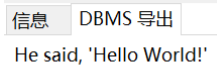
\includegraphics[width=0.3\textwidth]{picture/字符串分隔符效果图.png}
    \captionsetup{hypcap=false}
    \captionof{figure}{字符串分隔符输出演示}
    \label{fig:字符串分隔符效果图}
  \end{minipage}
\end{center}
\section{类型声明:\%TYPE属性}
为了避免这种变量数据类型和精度的硬编码(即数据类型和精度必须显式定义),PL/SQL引入\%TYPE属性。程序员(开发人员)可以使用\%TYPE属性按照之前已经声明过的变量或数据库的列来声明一个变量。当存储在一个变量中值来自于数据库中的表时,使用\%TYPE属性来声明这个变量时再适合不过的了。

\subsubsection{使用语法}
\begin{enumerate}
  \item 标识符\ 表名.列名\%TYPE
  \item 标识符\ 定义好的变量\%TYPE
\end{enumerate}
\subsubsection{案例}
\begin{plsql}
DECLARE
  v_data emp.data%TYPE
  v_Month_Value NUMBER(6,4) := 3.25
  v_Year_Value v_Month_Value%TYPE := 4.40
\end{plsql}
好处:
\begin{enumerate}
  \item 可以不知道emp表中的data列或v\_Month\_Value的数据类型和精度就直接使用对应类型。
  \item 当emp的data列或者v\_Month\_Value的数据类型和精度发生变化时,v\_data和v\_Year\_Value也会随之变化。
\end{enumerate}

\chapter{词法单元}
与其他程序设计语言一样,构成任何PL/SQL程序块的最基本单元的程序部件是词法单元。
一个词法单元就是一个字符序列,其中字符可以是字母、数字、特殊字符、空格、制表字符(tabs)、回车符、符号。

词法单元(位)又可以进一步划分成标识符、定界符、文字和注释四大类:
\begin{description}
  \item[标识符(Identifiers)] 标识符是命名的PL/SQL对象。
  \item[定界符(Delimiters)] 定界符是一些具有特殊含义的符号,其本身也经常被用作词法单元或语句的分隔符。
  \item[文字(Literals)] 任何赋予一个变量的值都是文字。
  \item[注释(Comments)] 是PL/SQL代码解释信息。
\end{description}

\section{标识符(Identifiers)}
标识符是用来命名数据库对象(如表、列、视图、过程、变量等)的名称。

其命名规则与变量命名规则完全相同,因此标识符也不能与保留关键字同名。{\bfseries\kaishu 如果使用保留关键字作为标识符名字或者标识符名字中包含了空格或要区分大小写},则必须在声明这个标识符时,将它用双引号括起来,如:  {\bfseries\kaishu “begin date” DATE}。

在之后使用这个标识符时也必须使用双引号。

\subsection{标识符命名惯例}

\begin{center}
  \begin{minipage}{\textwidth}
    \centering % 居中对齐
    \begin{tabular}{|c|c|c|} % 三列,居中对齐,列之间用竖线分隔
      \hline % 画水平线
      \textbf{标识符} & \textbf{命名惯例}  & \textbf{例子} \\
      \hline
      游标 & name\_cursor & emp\_cursor \\
      异常 & e\_name & e\_invalid\_product \\
      PL/SQL表类型 & name\_table\_type & ename\_table\_type \\
      PL/SQL表类型的变量 & name\_table  & ename\_table \\
      记录类型 & name\_record\_type & emp\_record\_type \\
      记录类型的变量 & name\_record & emp\_record \\
      \hline
    \end{tabular}
    \captionsetup{hypcap=false}
    \captionof{table}{标识符命名惯例表}
    \label{tab:标识符命名惯例} % 用于交叉引用的标签
  \end{minipage}
\end{center}

\section{定界符(Delimiters)}
定界符是用于界定代码块、语句、变量等元素范围的符号。在PL/SQL中,常见的定界符包括分号(;)、引号(')和双引号('')等。
\subsection{简单定界符}
简单定界符通常只有一个符号。

\begin{center}
  \begin{minipage}{\textwidth}
    \centering % 居中对齐
    \begin{tabular}{|c|c|} % 三列,居中对齐,列之间用竖线分隔
      \hline % 画水平线
      \textbf{操作符} & \textbf{含义}  \\
      \hline
      + & 加法运算符  \\
      - & 减法运算符  \\
      * & 乘法运算符  \\
      / & 除法运算符  \\
      = & 相等操作符  \\
      @ & 远程访问符  \\
      \hline
    \end{tabular}
    \captionsetup{hypcap=false}
    \captionof{table}{简单定界符表}
    \label{tab:简单定界符} % 用于交叉引用的标签
  \end{minipage}
\end{center}

\subsection{组合定界符}
组合定界符由二个符号组成。

\begin{center}
  \begin{minipage}{\textwidth}
    \centering % 居中对齐
    \begin{tabular}{|c|c|} % 三列,居中对齐,列之间用竖线分隔
      \hline % 画水平线
      \textbf{操作符} & \textbf{含义}  \\
      \hline
      ||  & 连接运算符  \\
      := & 赋值操作符  \\
      !=  & 不等运算符  \\
      <> & 不等运算符  \\
      /*\ */ & 开始/结束注释定界符  \\
      --  & 单行注释符  \\
      \hline
    \end{tabular}
    \captionsetup{hypcap=false}
    \captionof{table}{组合定界符表}
    \label{tab:组合定界符} % 用于交叉引用的标签
  \end{minipage}
\end{center}

\section{文字(Literals)}
任何赋予一个变量的值都是文字,即任何不是标识符的字符、数字、布尔或日期值都是文字。

文字可分为以下四类:
\begin{enumerate}
  \item \textbf{字符文字}:字符文字也叫字符串文字,字符串文字的数据类型只能是CHAR或VARCHAR2,如“社会核心价值观”、“中国梦”等。
  \item \textbf{数字文字}:一个数字文字就是一个正整数或实数,如“123”、“123.45”。
  \item \textbf{布尔文字}:赋予布尔变量的值是布尔文字,其值为TRUE、FALSE和NULL。
  \item \textbf{日期文字}:一个日期文字就是一个有效的日期类型数据,如9-mar-2022。
\end{enumerate}

\section{注释(Comments)}
如果只注释一行:那么直接使用{-}{-}。

如果注释的不止一行:那么使用符号 /* 和 */作为注释操作符。

\section{程序设计指导原则}
Oracle推荐在编写PL/SQL程序代码时应该遵循的大小写规范。利用这些大小写规范可以很容易区分关键字和对象,以增加项目的协同性和开发难度。

\begin{center}
  \begin{minipage}{\textwidth}
    \centering % 居中对齐
    \begin{tabular}{|c|c|c|} % 三列,居中对齐,列之间用竖线分隔
      \hline % 画水平线
      \textbf{种类} & \textbf{大小写}  & \textbf{例子} \\
      \hline
      SQL语句关键字 & 大写 & SELECT、FROM、UPDATE \\
      PL/SQL语句关键字 & 大写 & BEGIN、END、DECLARE \\
      数据类型 & 大写 & BOOLEAN、NUMBER \\
      标识符和参数 & 小写 & v\_job、g\_job、emp\_cursor \\
      数据库中的表和列 & 小写 & customers、empno、sal、dname \\
      \hline
    \end{tabular}
    \captionsetup{hypcap=false}
    \captionof{table}{大小写规范表}
    \label{tab:大小写规范} % 用于交叉引用的标签
  \end{minipage}
\end{center}

\chapter{运算符}

\section{基本运算符}
PL/SQL语言中的运算符与SQL语言中的基本相同:
\begin{enumerate}
  \item 算术(Arithmetic)运算符:+ - * / \%
  \item 比较(Comparison)运算符:= !=/<> < <= > >=
  \item 逻辑(Logical)运算符:AND/\&\& OR/|| NOT/!
  \item 位(Bitwise)运算符:AND OR XOR NOT
  \item 赋(Assignment)值运算符::=
  \item 串接|连接(Concatenation)运算符 :||
  \item 控制操作顺序的符号:()
  \item 模式匹配运算符:LIKE NOT LIKE
  \item 成员关系运算符:IN BETWEEN
  \item 等
\end{enumerate}
\section{空值运算}
可使用{\bfseries\kaishu Variable IN NULL}判断是否为NULL,如果返回值为true说明是NULL。

在操作空值(NULL)时,需要牢记:
\begin{itemize}
  \item 在{\bfseries\kaishu 比较表达式}(如<>)中只要有空值,其结果总是空值;
  \item 对一个空值进行NOT运算,其结果还是空值;
  \item 在条件(分支)语句中,如果条件为NULL,与这个条件相关的语句序列将不会执行。
\end{itemize}



\chapter{预定义函数}
为了方便地使用Oracle数据库,Oracle SQL提供了大量的可以在SQL语句中使用预定义函数,实际上这些函数增强了SQL语言功能。这些函数的{\bfseries\kaishu 绝大多数}在PL/SQL表达式中也是有效的,如单行数字函数、单行字符函数、数据类型转换函数、日期函数、Timestamp函数、GREATEST、LEAST函数等。

注意:{\bfseries\kaishu 分组函数}(如AVG、MIN、MAX、COUNT、SUM、STDDEV和VARIANCE函数等)依旧只能在SQL语句中使用,不能用于PL/SQL的表达式中。

\section{单行数字函数}
以下为常用单行数字函数:
\begin{description}
  \item[三角函数] 如:SIN、ASIN、SINH、COS、ACOS、COSH、TAN、ATAN、TANH。
  \item[ABS(X)] 绝对值。
  \item[BITAND(X,Y)] 对两个数字进行按位与(AND)运算,得到的结果是一个新的整数。
  \item[CEIL(X)] 返回大于或等于X的最小整数。
  \item[FLOOR(X)]  返回小于或等于X的最大整数。
  \item[exp(X)] 返回e的x次幂。
  \item[LN(X)] 返回X的自然对数。
  \item[POWER(X,Y)] 返回X的Y次幂。
  \item[SQRT(X)] 返回X的平方根。
  \item[ROUND(\textup{X[,Y]})] 返回对x取整的结果,其中y为可选,说明对第几位小数处取整。
\end{description}
\section{单行字符函数}
以下为常用单行字符函数:
\begin{description}
  \item[concat(m,n)] 将m和n连接起来,并返回连接后的字符串。
  \item[initcap(n)] 将n中的第一个字母转换成大写。
  \item[instr(x,y,m,n)] 在字符串x中查找字符串y出现的位置,m是搜索开始的位置,n是指定第n次字符串y出现的位置。
  \item[length(n)] 求字符串n的长度。
  \item[lower(n)] 求字符串n的长度。
  \item[lpad(x,n,y)] 在字符串x的左边补齐字符y,得到总长度为n个字符的字符串。
  \item[rpad(x,n,y)] 在字符串x的右边补齐字符y,得到总长度为n个字符的字符串。
  \item[\textup{trim([LEADING | TRAILING | BOTH] trim\_character FROM source\_string)}]  \ \\去除字符串source\_string两端(或左侧、右侧)的指定字符trim\_character。
  \item[ltrim(x,y)] 去除字符串x左侧的指定字符y。
  \item[rtrim(x,y)] 去除字符串x右侧的指定字符y。
\end{description}

\section{数据类型转换函数}

PL/SQL支持动态数据类型转换,分为两大类:{\bfseries\kaishu 隐含转换}和{\bfseries\kaishu 显示转换}。隐含转换发生在混合使用多种数据类型的语句中,PL/SQL会尝试自动转换数据类型,如字符型和数字型之间、字符型和日期型之间。显示转换则需要使用内置的转换函数,例如TO\_CHAR、TO\_DATE、TO\_NUMBER和TO\_TIMESTAMP,用于将一个值从一种数据类型转换为另一种数据类型。

以下为常用的数据类型转换函数:
\begin{enumerate}
  \item {\bfseries\kaishu TO\_NUMBER(expr, [format\_mask], [nls\_params])}:其中 expr 是要转换的表达式,\\format\_mask 是可选的格式掩码,nls\_params 是可选的国家语言设置。
  \item {\bfseries\kaishu TO\_CHAR(expr, [format\_mask], [nls\_params])}:其中 expr 是要转换的表达式,format\_mask 是可选的格式掩码,nls\_params 是可选的国家语言设置。
  \item {\bfseries\kaishu TO\_DATE(char\_string, [format\_mask], [nls\_params])}:其中 char\_string 是要转换的字符串,format\_mask 是可选的格式掩码,nls\_params 是可选的国家语言设置。
  \item {\bfseries\kaishu CAST(num AS type)}进行显式的数据类型转换,用于将一个数据类型转换为另一个数据类型,如\textbf{str := CAST(num AS VARCHAR2(20));}。
\end{enumerate}

\section{日期函数}
以下为常用的日期函数:
\begin{description}
  \item[SYSDATE] 返回当前系统日期和时间。
  \item[TO\_DATE] 将字符串转换为日期类型,\\如c{\bfseries\kaishu onverted\_date := TO\_DATE('2023-01-01', 'YYYY-MM-DD');}。
  \item[MONTHS\_BETWEEN] 计算两个日期之间的月份差,\\如\textbf{months\_diff := MONTHS\_BETWEEN(date2, date1);}。
  \item[ADD\_MONTHS] 在给定日期上增加指定的月数,\\如\textbf{result\_date := ADD\_MONTHS(start\_date, 3);}。
  \item[LAST\_DAY] 本月的最后一天。
  \item[NEXT\_DAY(start\_date, day\_of\_week)] 找到指定日期之后的下一个指定星期几的日期,\\day\_of\_week 是星期的缩写,例如 'MON' 表示星期一,'TUE' 表示星期二,以此类推。
  \item[\textup{ROUND(date\_expression [, format\_mask])}] 将日期四舍五入到指定的精度。\\如\textbf{rounded\_date := ROUND(current\_date, 'MONTH');}。
  \item[\textup{TRUNC(date\_expression [, format\_mask]);}] 截断日期到指定的精度,类似ROUND函数。
\end{description}
\section{CHR函数}
CHR(integer)函数的作用是将所给的数字换成对应的ASCII码字符(因为有一些字符无法用键盘输入)。

如:
\begin{itemize}
  \item CHR(9) -- 制表符
  \item CHR(10) -- 换行符
  \item CHR(13) -- 回车符
  \item CHR(32) -- 空格符
  \item CHR(34) -- 双引号
  \item CHR(39) -- 单引号
\end{itemize}

\chapter{序列}
\section{序列概念}
在SQL中,序列(Sequence)是一种数据库对象,用于生成唯一的数字值。它通常用于为表的主键列生成唯一标识符。序列是数据库中的一种生成器,提供了一种自动递增或递减的数字值生成方式。

创建序列的语法:
\begin{plsql}[caption=创建序列语法]
CREATE SEQUENCE sequence_name
  [INCREMENT BY n]
  [START WITH n]
  [MAXVALUE n | NOMAXVALUE]
  [MINVALUE n | NOMINVALUE]
  [CYCLE | NOCYCLE]
  [CACHE n | NOCACHE];
\end{plsql}

各参数的含义:
\begin{enumerate}
  \item \textbf{INCREMENT BY: }指定序列的增量,默认为1。
  \item \textbf{START WITH: }指定序列的起始值,默认为1。
  \item \textbf{MAXVALUE和MINVALUE: }分别指定序列的最大值和最小值。
  \item \textbf{CYCLE | NOCYCLE: }指定是否循环序列值,如果达到最大值后再次从最小值开始(或相反)。
  \item \textbf{CACHE | NOCACHE: }指定是否缓存序列值,以提高性能。
\end{enumerate}

\section{PL/SQL中序列的操作} 
\subsection{NEXTVAL}
{\bfseries\kaishu NEXTVAL }函数用于获取序列的下一个值。{\bfseries\kaishu 每次调用 NEXTVAL 都会获取序列的下一个值,并且序列的计数器会递增(更新序列)。}
\begin{plsql}[caption=NEXTVAL示例代码]
DECLARE
  next_id NUMBER;
BEGIN
  next_id := your_sequence_name.NEXTVAL;
  DBMS_OUTPUT.PUT_LINE('Next ID: ' || next_id);
END;
\end{plsql}
\subsection{CURRVAL}
{\bfseries\kaishu CURRVAL} 函数用于获取序列的当前值。
\begin{plsql}[caption=CURRVAL示例代码]
DECLARE
  current_id NUMBER;
BEGIN
  current_id := your_sequence_name.CURRVAL;
  DBMS_OUTPUT.PUT_LINE('Current ID: ' || current_id);
END;
\end{plsql}
\chapter{SELECT}
\section{INTO}
在PL/SQL的SELECT语句中增加了INTO子句。通过SELECT子句提取(查找到的)数据(表中列的值),而通过INTO子句将提取的数据存放在PL/SQL变量中。

\begin{plsql}[caption=SELECT示例代码]
SELECT 查询列表
INTO {变量名[,变量名]… | 记录名}
FROM 表
[WHERE 条件表达式];
\end{plsql}
\begin{description}
  \item[查询列表(select\_list)] 为一个或多个(至少一个)列名、SQL表达式、SQL单行函数或SQL分组函数。
  \item[变量名(Variable\_name)] 存储获取值的PL/SQL标量变量。
  \item[记录名(record\_name)] 存储多个取值的PL/SQL记录类型的变量。
  \item[表(Table)] 数据库中的表名(从中提取数据的表)。
  \item[条件表达式(condition)] 由列名、表达式、常量和比较操作符组成的表达式,其中可以包括PL/SQL变量和常量。
\end{description}

注意事项:
\begin{enumerate}
  \item 每一个SQL语句必须有分号(;)。
  \item INTO子句是{\bfseries\kaishu 强制性}的(必须存在),并只能放在SELECT子句和FROM子句之间。
  \item 每一个从表中提取的值{\bfseries\kaishu 必须存入一个PL/SQL的变量中}(通过INTO),而每一个变量都必须在使用前声明过;此外必须为所选择的项(列或表达式)指定一个变量,顺序要对应
  \item 在INTO子句中的变量的个数必须与查询列表中数据库列的个数完全相同,并且每一个变量数据类型和精度一定与对应位置的列兼容。
  \item 使用 SELECT INTO 语句时,{\bfseries\kaishu 确保查询返回的结果只有一行}。如果查询返回多行(此时应该使用BULK COLLECT INTO代替INTO)或没有数据,PL/SQL 将引发 TOO\_MANY\_ROWS 或 NO\_DATA\_FOUND 异常。
  \item 可以在SQL语句中使用分组函数。
  \item INTO子句中使用的变量可以PL/SQL变量,也可以是宿主变量(如绑定变量)。
\end{enumerate}

\begin{plsql}[caption=INTO案例代码]
DECLARE
  v_deptno dept.deptno%TYPE;
  v_loc VARCHAR2(38);
BEGIN
  SELECT deptno,loc
  INTO v_deptno, v_loc
  FROM dept
  WHERE dname = 'ACCOUNTING';
END;
/
\end{plsql}

\section{变量与列同名问题}
Oracle系统在执行PL/SQL中嵌入的SQL语句时是按照标识符的优先次序来处理标识符的,所以如果PL/SQL变量与列名同名,则可能造成程序的二义性。Oracle的处理变量、参数、表和列的优先级如下:
\begin{enumerate}
  \item PL/SQL首先检查数据库表中{\bfseries\kaishu 列}的名字
  \item 数据库表中列的名字优先于{\bfseries\kaishu 本地变量名}
  \item 本地变量名和形式参数名优先于数据库的{\bfseries\kaishu 表}名
\end{enumerate}

列名(Column Name)>变量名(Variable Name) >表名(Table Name)

\chapter{DML}
\section{概述}
在PL/SQL程序块中不能直接使用数据定义语言(DDL)的语句(如不能使用CREATE TABLE、ALTER TABLE或者TRUNCATE TABLE等),并且也不能直接使用数据控制语言(DCL)的语句(如不能使用GRANT或者REVOKE语句)。

注意:EXECUTE IMMEDIATE 是用于执行动态 SQL 的语句,这允许PL/SQL程序在运行时动态生成 SQL 语句并执行(动态 SQL 允许以字符串形式构建 SQL 语句)。在使用动态 SQL 的情况下,PL/SQL 通过动态 SQL 获得了一种间接执行 DDL 和 DCL 操作的方式。

DDL和DML的区别:
\begin{enumerate}
  \item DDL代表数据定义语言,而DML代表数据操作语言。
  \item DDL中常用的命令有:create,drop,alter,truncate和rename 而 DML中常用的命令有:insert,update,delete和select等等。
  \item DDL命令会影响整个数据库或表而DML命令会影响表中的一个或多个记录。
  \item 带有DDL命令的SQL语句无法回滚;带有DML命令的SQL语句可以回滚。
\end{enumerate}

PL/SQL中存在4类DML语言:
\begin{enumerate}
  \item {\bfseries\kaishu INSERT语句:}往一个表中添加一行新数据。
  \item {\bfseries\kaishu UPDATE语句:}更改一个表中现有的数据行。
  \item {\bfseries\kaishu DELETE语句:}从一个表中移除数据行。
  \item {\bfseries\kaishu MERGE语句:}从一个表中选择数据行以修改或插入到另一个表。
\end{enumerate}

\section{DML代码示例}
\subsection{INSERT}
\begin{plsql}[caption=INSERT代码示例]
BEGIN
  INSERT INTO dept(deptno, dname, loc);
  VALUES (deptid_sequence.NEXTVAL, '燕城苑','天通苑');
END;
/
\end{plsql}
使用序列deptid\_sequence的NEXTVAL产生新记录的deptno。

\subsection{UPDATE}
\begin{plsql}[caption=UPDATE代码示例]
DECLARE
  v_sal_increase emp.sal%TYPE := &p_sal_increase;
BEGIN
  UPDATE emp
  SET sal = sal + v_sal_increase
  WHERE job = 'CLERK';
END;
/
\end{plsql}

\subsection{DELETE}
\begin{plsql}[caption=DELETE代码示例]
DECLARE
  v_job emp.job%TYPE := '&p_job';
  v_sal emp.sal%TYPE := &p_sal;
BEGIN
  DELETE FROM emp_pl
  WHERE job = v_job
  AND sal > v_sal;
END;
/
\end{plsql}

\section{MERGE}
利用MERGE语句,可以根据设定的条件来决定对表的操作是修改、插入还是删除,从而避免了使用多个DML语句。

\subsection{MERGE基本语法}
\begin{plsql}[caption=MERGE语法]
MERGE INTO target_table USING source_table
ON (condition)
WHEN MATCHED THEN
-- 更新操作
WHEN NOT MATCHED THEN
-- 插入操作
\end{plsql}

\begin{description}
  \item[INTO 子句] 说明正在修改或插入的目标表
  \item[USING 子句] 标识要修改或插入的数据源,既可以是表,也可以是视图
  \item[ON 子句]  定义MERGE语句是进行修改操作还是进行插入操作的条件
  \item[WHEN MATCHED THEN]  定义当条件满足时所做的操作
  \item[WHEN NOT MATCHED THEN] 定义当条件不满足时所做的操作
\end{description}

\subsection{MERGE示例代码}
\begin{plsql}[caption=MERGE示例代码1]
MERGE INTO employees target
USING employees_backup source
ON (target.employee_id = source.employee_id)
WHEN MATCHED THEN
  UPDATE SET target.salary = source.salary
WHEN NOT MATCHED THEN
  INSERT (employee_id, salary) VALUES
  (source.employee_id, source.salary);
\end{plsql}

\begin{plsql}[caption=MERGE示例代码2]
BEGIN
  MERGE INTO copy_emp c
  USING emp e
  ON (c.empno = e.empno)
  WHEN MATCHED THEN
    UPDATE SET
      c.empno = e.empno,
      c.ename = e.ename,
      c.job = e.job,
      c.mgr = e.mgr,
      c.hiredate = e.hiredate,
      c.sal = e.sal,
      c.comm = e.comm,
      c.deptno = e.deptno
  WHEN NOT MATCHED THEN
    INSERT (empno, ename, job, mgr, hiredate, sal, comm, deptno) 
    VALUES (e.empno, e.ename, e.job, e.mgr, e.hiredate, e.sal, e.comm, e.deptno);
END;
/
\end{plsql}

\chapter{条件语句}
\section{布尔条件}
如果要构建一个复杂的布尔条件,需要使用逻辑运算符AND(逻辑与/逻辑乘)、OR(逻辑加/逻辑或)或NOT(逻辑非)将简单的布尔条件组合在一起。

AND和OR用于把两个条件组合在一起最后产生一个结果,其语法是:

{\bfseries\kaishu 条件1\ 逻辑运算符\ 条件2;}

\subsection{各类AND运算结果}
思路:有F就是F,否则有N就是N。
\begin{center}
  \begin{minipage}{\textwidth}
    \centering
    \begin{tabular}{|c|c|c|c|} 
      \hline % 画水平线
      \textbf{运算结果}   &   \textbf{T}  &   \textbf{F}  &   \textbf{NULL} \\
      \hline
      \textbf{T}          &   T AND T = T & T AND F = F  &  T AND N = N \\
      \hline
      \textbf{F}          &   F AND T = F & F AND F = F  &  F AND N = F \\
      \hline
      \textbf{NULL}       &   N AND T = N & N AND F = F  &  N AND N = N \\
      \hline
    \end{tabular}
    \captionsetup{hypcap=false}
    \captionof{table}{各类AND运算结果表}
    \label{tab:各类AND运算结果表} % 用于交叉引用的标签
  \end{minipage}
\end{center}

\subsection{各类OR运算结果}
思路:有T就是T,否则有N就是N。
\begin{center}
  \begin{minipage}{\textwidth}
    \centering
    \begin{tabular}{|c|c|c|c|} 
      \hline % 画水平线
      \textbf{运算结果}   &   \textbf{T}  &   \textbf{F}  &   \textbf{NULL} \\
      \hline
      \textbf{T}          &   T OR T = T & T OR F = T  &  T OR N = T \\
      \hline
      \textbf{F}          &   F OR T = T & F OR F = F  &  F OR N = N \\
      \hline
      \textbf{NULL}       &   N OR T = T & N OR F = N  &  N OR N = N \\
      \hline
    \end{tabular}
    \captionsetup{hypcap=false}
    \captionof{table}{各类OR运算结果表}
    \label{tab:各类OR运算结果表} % 用于交叉引用的标签
  \end{minipage}
\end{center}
\subsection{各类NOT运算结果}
\begin{enumerate}
  \item NOT T = F
  \item NOT F = T
  \item NOT NULL = N
\end{enumerate}
\section{IF语句}
在PL/SQL中最常见的分支(条件)语句就是IF语句。PL/SQL语言的IF语句的结构与其它结构化语言中IF语句的结构完全相似。

\subsection{IF 语句语法}
\begin{plsql}[caption=IF语法]
IF 条件 THEN
  statements
[ELSIF 条件 THEN
  statements;]
[ELSE
  statements;]
END IF;
\end{plsql}

\begin{plsql}[caption=IF语法示例1]
IF condition THEN
  -- 仅在条件为真时执行的代码块
END IF;

IF condition1 THEN
  -- 在条件1为真时执行的代码块
ELSIF condition2 THEN
  -- 在条件2为真时执行的代码块
END IF;

IF condition1 THEN
  -- 在条件1为真时执行的代码块
ELSE
  -- 在条件1不为真时执行的默认代码块
END IF;
\end{plsql}

\begin{description}
  \item[条件(condition)] 是一个返回True、False或NULL的布尔变量或表达式
  \item[THEN] 引出一个子句
  \item[Statements] 可以是一个或多个PL/SQL或SQL语句
  \item[ELSIF] 引入一个布尔表达式的关键字
  \item[ELSE] 与之前所有的条件都不成立时引入默认子句
  \item[END IF] IF语句结束的标志,END IF后需要接 \textbf{;} 以结束
\end{description}

\subsection{IF 语句示例}
\begin{plsql}
DECLARE
  v_age number := &p_age;
  v_gender CHAR(1) := '&p_sex';
BEGIN
  IF (v_age BETWEEN 18 AND 35) AND (v_gender = 'F') 
  THEN
    DBMS_OUTPUT.PUT_LINE('符合研究生入学年龄');
  END IF;
END;
/
\end{plsql}
运行结果:

{\bfseries\kaishu 输入 p\_age 的值: 22

输入 p\_sex 的值: F

符合研究生入学年龄}

\subsection{注意}
\begin{enumerate}
  \item 尽管可以使用IF语句中嵌套一个或多个IF语句的方式构造出多路分支语句,但是这样做的结果会使程序的逻辑变得复杂并且易读性下降。因此,在实际工作中应该尽量避免使用IF语句的嵌套,而使用ELSIF子句。
  \item PL/SQL的逻辑表达式求值(又称最小化求值)是一种逻辑运算符策略。只有当第一个运算数的值无法确定逻辑运算结果时,才对第二个运算数进行求值。
\end{enumerate}

\section{CASE表达式}
\subsection{CASE 表达式语法}
\begin{plsql}[caption=带选择器]
CASE selector
  WHEN 表达式1 THEN 结果1
  WHEN 表达式2 THEN 结果2
  …
  WHEN 表达式N THEN 结果N
  [ELSE 结果 N+1]
END;
\end{plsql}

PL/SQL还提供了一种搜索CASE表达式。这种搜索CASE表达式没有选择器,而是WHEN子句本身包含了产生一个布尔值的搜索条件,因此WHEN子句表达式不能产生其他任何类型的值。

\begin{plsql}[caption=不带选择器]
CASE
  WHEN 表达式1 THEN 结果1
  WHEN 表达式2 THEN 结果2
  …
  WHEN 表达式N THEN 结果N
  [ELSE 结果 N+1]
END;
\end{plsql}
\subsection{CASE 表达式示例}
\begin{plsql}[caption=CASE示例代码]
DECLARE
  v_degree CHAR(1) := UPPER('&p_degree');
  v_description VARCHAR2(250);
BEGIN
  v_description := 
    CASE v_degree
      WHEN 'B' THEN '此人拥有学士学位。'
      WHEN 'M' THEN '此人拥有硕士学位。'
      WHEN 'D' THEN '此人拥有博士学位。'
      ELSE '此人拥有壮士学位。'
    END;
  DBMS_OUTPUT.PUT_LINE(v_description);
END;
/
\end{plsql}
运行结果:

{\bfseries\kaishu 输入 p\_degree 的值: B

此人拥有学术学位。}

CASE表达式的结果(返回值)可以是任何数据类型,只要与要赋值的变量的数据类型兼容(匹配)就可以。

\section{CASE语句}
CASE表达式测试条件并返回一个值,而CASE语句测试条件并执行一个操作。一个CASE语句可以是一个完整的PL/SQL程序块。CASE语句必须以“END CASE;”结束,而CASE表达式必须以“END;”结束。
\subsection{CASE 语句示例代码}
\begin{plsql}
DECLARE
  v_degree CHAR(1) := UPPER('&p_degree');
BEGIN
  CASE v_degree
    WHEN 'B' THEN 
      DBMS_OUTPUT.PUT_LINE('此人拥有学士学位。');
    WHEN 'M' THEN 
      DBMS_OUTPUT.PUT_LINE('此人拥有硕士学位。');
    WHEN 'D' THEN '此人拥有博士学位。'
      DBMS_OUTPUT.PUT_LINE('此人拥有博士学位。');
    WHEN 'X' THEN
      DBMS_OUTPUT.PUT_LINE('此人拥有壮士学位。');
  END CASE;
END;
/
\end{plsql}
运行结果:

{\bfseries\kaishu 输入 p\_degree 的值: B

此人拥有学术学位。}

\subsection{使用CASE语句取代DECODE}
利用CASE表达式或CASE语句来取代SQL函数的DECODE可以使程序变得更加清晰。
\begin{plsql}[caption=DECODE函数]
v_grade := DECODE(v_score,
  90, 'A',
  80, 'B',
  70, 'C',
  'D'
);
\end{plsql}
\begin{plsql}[caption=CASE表达式]
CASE v_score
  WHEN 90 THEN v_grade := 'A'
  WHEN 80 THEN v_grade := 'B'
  WHEN 70 THEN v_grade := 'C'
  ELSE v_grade := 'D'
END CASE;
\end{plsql}

\section{GOTO}
虽然在PL/SQL程序设计语言中有GOTO语句,但是许多PL/SQL语言的教材并不介绍这一个极具有争议的语句。GOTO语句一直是批评和争论的焦点,主要是负面影响是使用GOTO语句使程序的可读性变差,甚至成为不可维护的“面条代码”。

语法:{\bfseries\kaishu GOTO 语句标号}

\subsection{用处}
\begin{enumerate}
  \item {\bfseries\kaishu 错误处理和清理:}有时,当在代码中发生错误时,需要跳转到一个错误处理和清理代码块。这个错误处理代码块通常包括关闭文件、释放资源、记录错误日志等操作。在这种情况下,使用GOTO语句可以让你跳转到错误处理部分,以确保资源得到释放,并记录错误信息。
  \item {\bfseries\kaishu 特定性能优化:}在某些特殊情况下,使用GOTO语句可以实现更高效的代码执行,特别是在循环或嵌套结构中。这通常需要精心考虑和测试,以确保性能的提高值得引入GOTO。
\end{enumerate}
\begin{plsql}[caption=错误处理示例代码]
BEGIN
  -- 一些代码
  -- 发生错误时跳转到错误处理部分
  IF error_condition THEN
    GOTO error_handler;
  END IF;
  -- 正常代码继续执行
  -- ...
  EXIT; -- 跳过错误处理部分
  
  <<error_handler>> -- 错误处理部分
  -- 执行清理操作、记录错误日志等
  -- ...
END;
/
\end{plsql}

\begin{plsql}[caption=性能提升示例代码(循环)]
DECLARE
  total_processed NUMBER := 0;
  max_iterations NUMBER := 1000000; -- 假设有一个很大的数据集
  iteration NUMBER := 0;
BEGIN
  <<main_loop>> -- 主循环
  IF iteration >= max_iterations THEN
    GOTO end_loop; -- 跳过剩余迭代
  END IF;
  -- 执行数据处理操作
  total_processed := total_processed + 1;
  iteration := iteration + 1;
  GOTO main_loop; -- 继续下一次迭代

  <<end_loop>> -- 结束循环
  DBMS_OUTPUT.PUT_LINE('处理完成,总共处理了 ' || total_processed || ' 条数据。');
END;
\end{plsql}

\chapter{循环语句}
所谓的循环就是多次重复一个语句或语句序列。PL/SQL提供了若干个循环结构以控制语句的重复执行。循环主要用于重复执行一些语句直到一个条件满足为止。在一个循环中必须要有一个退出条件,否则就是一个死循环。

PL/SQL提供一下三种类型的循环结构:
\begin{enumerate}
  \item {\bfseries\kaishu 基本循环:}执行无条件的重复操作。
  \item {\bfseries\kaishu WHILE循环:}执行基于一个条件的重复操作。
  \item {\bfseries\kaishu FOR循环:}执行基于一个计数器的重复操作。
\end{enumerate}

建议:
\begin{itemize}
  \item 当语句在循环中至少要执行一次时,一般使用基本循环。
  \item 如果在每次开始重复时都必须测试条件,一般使用WHILE循环。
  \item 如果重复次数为已知,一般使用FOR循环。
\end{itemize}

\section{基本循环}
\subsection{基本循环语法}
最简单的循环语句就是
基本循环,它是由包含在\textbf{LOOP}和\textbf{END LOOP}关键字之间的一个语句序列构成。每次执行的流程达到END LOOP语句时,程序的控制就是转到LOOP结构的最上面。基本循环运行它的语句至少执行一次,即使在进入这个循环时EXIT条件已经满足,也要执行一次。如果没有EXIT语句,基本循环是一个死循环。

语法:
\begin{plsql}[caption=基本循环语法]
LOOP -- 定界符
  statement; -- 一个或多个语句
  …
  EXIT [WHEN condition]; -- 退出语句(EXIT语句)
END LOOP; -- 定界符
\end{plsql}

\begin{description}
  \item[Condition] 一个布尔变量或者布尔表达式。
  \item[Statement] 一个或多个SQL语句或一个或多个PL/SQL语句。
\end{description}

\subsection{基本循环示例}
\begin{plsql}[caption=基本循环示例代码]
DECLARE
  v_empno emp_pl.empno%TYPE;
  v_deptno emp_pl.deptno%TYPE := &p_deptno;
  v_sal emp_pl.sal%TYPE := &p_sal;
  v_hiredate emp_pl.hiredate%TYPE := SYSDAYE;
  v_job emp_pl.job%TYPE := '&p_job';
  v_counter NUMBER(2) := 1;
  v_max_num NUMBER(2) := &P_max_num;
BEGIN
  SELECT MAX(empno) INTO v_empno FROM emp_pl;
  LOOP
    INSERT INTO emp_pl(empno, hiredate, job, sal, deptno)
    VALUES((v_empno + v_counter), v_hiredate, v_job, v_sal, v_deptno);
    v_counter := v_counter + 1;
    EXIT WHEN v_counter > v_max_num;
  END LOOP;
END;
\end{plsql}

\section{WHILE循环}
\subsection{WHILE 循环语法}
PL/SQL还提供了一种与基本(LOOP)循环相似的WHILE LOOP循环语句,但是使用WHILE循环条件为真(TRUE)时重复执行循环体中的语句,而当条件不再是TRUE(F或N)时退出循环。

循环的条件是在每次重复开始时测试,这种循环是在条件为FALSE或NULL终止。WHILE LOOP的循环语句语法如下:
\begin{plsql}[caption=WHILE循环语法]
WHILE 条件 LOOP
  语句1;
  语句2;
  …
END LOOP;
\end{plsql}

在WHILE LOOP循环语句中,循环的条件必须放在WHILE和LOOP两个关键字之间,而循环的条件是在每次重复开始时测试的。与LOOP循环语句相同,在WHILE LOOP循环语句中所包含的语句既可以是PL/SQL语句也可以是SQL语句。

\subsection{WHILE 循环示例}
\begin{plsql}[caption=WHILE循环示例代码]
DECLARE
  v_deptno dept.deptno%TYPE;
  v_loc dept.loc%TYPE := '&p_loc';
  v_counter NUMBER(2) := 1;
  v_max_num NUMBER(2) := &p_max_num;
BEGIN
  WHILE v_counter <= v_max_num LOOP;
    INSERT INTO dept_pl(deptno, loc)
    VALUES(deptid_sequence.NEXTVAL, v_loc);
    v_counter := v_counter + 1;
  END LOOP;
END;
/
\end{plsql}

\section{FOR循环}
\subsection{FOR 循环语法}
For循环具有与基本循环一样的通用结构,不过For循环在LOOP关键字之前有一个控制语句用来设置PL/SQL程序执行的重复次数。For循环具有如下特性:
\begin{enumerate}
  \item 使用FOR循环简化了对重复次数的测试.
  \item 不用声明计数器,它是隐含声明的.
  \item 在语法上需要说明下限和上限.
\end{enumerate}

语法:
\begin{plsql}[caption=FOR循环语法]
FOR counter IN [REVERSE] lower_bound..upper_bound LOOP
  statement1;
  statement2;
  …
END LOOP;
\end{plsql}
\begin{description}
  \item[counter] 是一个隐含声明的整型数,其值在循环的每次重复时自动增加或减少(默认是增加)。
  \item[REVERSE] 指定计数器每次重复时是从上限到下限递减(默认是从下限到上限)。
  \item[lower\_bound] 下限。
  \item[upper\_bound] 上限。
\end{description}

语句序列每执行一次,计数器默认加1。除了整数之外,循环范围的下限和上限还可以是文字、变量和表达式,但是必须可以转换成整数的数据类型。如果下限和上限不是整数,PL/SQL按四舍五入的方法将其转为整数。因此,13/2和17/3都是有效的上限或下限值。

\subsection{FOR 循环示例}
\begin{plsql}[caption=FOR循环示例代码]
DECLARE
  v_deptno dept.deptno%TYPE;
  v_loc dept.loc%TYPE := '&p_loc';
  v_max_num NUMBER(2) := &p_max_num;
BEGIN
  FOR i IN 1..v_max_num LOOP
    INSERT INTO dept_pl(deptno, loc);
    VALUES(deptid_sequence.NEXTVAL, v_loc);
  END LOOP;
END;
/
\end{plsql}

使用FOR循环时应该遵守的规则:
\begin{enumerate}
  \item 只在循环中引入计数器,计数器在循环外没有定义。
  \item {\bfseries\kaishu 不要为计数器赋值},即不要将计数器变量放在赋值运算符的左边。
  \item 上限和下限都不应该为空值 NULL。
\end{enumerate}

\section{循环的嵌套与标号}
\subsection{介绍}
循环体本身也是一个PL/SQL程序块,所以PL/SQL的循环同样可以嵌套,而且可以进行多层嵌套、将基本循环、WHILE循环和FOR循环彼此之间混合嵌套。

一个被嵌套的循环的结束并不结束包含它的循环(除非出现异常)。不过,可以使用标号以区分不同的块和循环体,并引用带有标号的EXIT语句直接退出外层循环。

标号的命名规则与其它标识符完全相同(在之前条件语句中,GOTO章节也用到了标号)。标号必须放在一个语句之前,既可以是在同一行,也可以是在单独的行。为基本循环加标号时,标号要放在关键字LOOP之前并用标号定界符 “<<”和“>>”括起来,如<<dog\_loop>>,其中dog\_loop为标号。在FOR循环和WHILE循环中,标号要放在关键字FOR或WHILE之前。

\subsection{循环的嵌套与标号示例}
程序有2个嵌套的FOR循环,用户利用代替变量输入一个正整数n,之后再外循环中的程序计算出1~n所有自然数之和。内循环计算所输入自然数的阶乘(n!)。
当i+j>4成立时,程序就跳转到Inner\_loop标号所再得语句。其中,i和j分别为外循环和内循环的计数。

\begin{plsql}[caption=嵌套循环示例代码]
  DECLARE
  v_t NUMBER := 0;
  v_f NUMBER := 1;
  v_num NUMBER := 10;
BEGIN
  <<Outer_Loop>>
  FOR i IN 1..v_num LOOP
    v_t := v_t + i;
    DBMS_OUTPUT.PUT_LINE('1~'||i||'自然数的总和是:'||v_t);
    <<Inner_Loop>>
    FOR j IN 1..v_num LOOP
      EXIT Inner_Loop WHEN i+j >4;
      v_f := v_f * j;
      DBMS_OUTPUT.PUT_LINE('自然数'||j||'的阶乘是:'||v_f);
    END LOOP;
    v_f := 1;
  END LOOP Outer_Loop;
END;
/
\end{plsql}

\section{CONTINUE}
\subsection{介绍}
Oracle 11g和Oracle 12c引入了CONTINUE语句,该语句能够使程序的控制转移到循环体中的下一次新循环或者直接离开循环。通常使用CONTINUE语句在主要的处理开始之前在一个循环内部过滤掉不需要的数据(和处理操作)。

\subsection{CONTINUE示例}
注意:此代码效果与嵌套循环示例代码效果相同。

\begin{plsql}[caption=CONTINUE示例代码]
DECLARE
  v_t NUMBER := 0;
  v_f NUMBER := 1;
  v_num NUMBER := 20;
BEGIN
  <<Outer_Loop>>
  FOR i IN 1..v_num LOOP
    v_f := 1;
    v_t := v_t + i;
    DBMS_OUTPUT.PUT_LINE('1~'||i||'自然数的总和是:'||v_t);
    <<Inner_Loop>>
    FOR j IN 1..v_num LOOP
      CONTINUE Outer_Loop WHEN i+j >4;
      v_f := v_f * j;
      DBMS_OUTPUT.PUT_LINE('自然数'||j||'的阶乘是:'||v_f);
    END LOOP;
  END LOOP Outer_Loop;
END;
/
\end{plsql}

\chapter{组合数据类型}
一个组合类型的变量可以存放多个变量类型的值或多个组合类型的值。

与标量数据类型不同,组合数据类型包含了内部结构(组件),一旦定义了一个数据类型,这个数据类型就可以重用——用来定义一个或多个组合类型变量。

PL/SQL语言中的组合数据类型可以分为以下几类:
\begin{enumerate}
  \item PL/SQL记录(records):将逻辑上相关的但是类型不同的数据当作一个逻辑单元来处理,{\bfseries\kaishu 一个PL/SQL记录可以包含多个不同类型的数据},如可以定义一个存储客户详细信息的记录。
  \item PL/SQL集合(collections):将一组(集合)数据当作一个单独的单元来处理。
  \begin{enumerate}
    \item INDEX BY表
    \item 嵌套表(Nested Table)
    \item 变长数组(VARRAY)
  \end{enumerate}
\end{enumerate}

PL/SQL记录和PL/SQL集合都是组合数据类型,在实际编程中选择的原则:
\begin{itemize}
  \item 如果要存储和操作的数据是逻辑上相关的但是具有不同的数据类型,一般使用PL/SQL记录。
  \item 如果要存储和操作的数据具有相同的数据类型,而且其数据类型本身又可以是组合类型,使用INDEX BY表。
\end{itemize}

\section{PL/SQL记录(records)}
\subsection{介绍}
所谓一个PL/SQL记录就是{\bfseries\kaishu 一组存储在若干字段中的相关联的数据}(类似对象),而记录中的每个字段都具有自己的名字和数据类型。

PL/SQL记录具有如下特性:
\begin{enumerate}
  \item 一定包含一个或多个被称为字段的组件,其组件是任何的标量、记录或INDEX BY表的数据类型。
  \item 在结构上与第三代语言(3GL)的记录相似。
  \item {\bfseries\kaishu 与数据库中表的行不同。}
  \item 每一个定义的记录可以根据实际需要有任意多个字段。
  \item 可以为记录赋初始值,也可以将记录定义为非空(NOT NULL),没有初始值的字段其初始值被初始化为空(NULL),也可以使用关键字DEFAULT为其定义初始值。
  \item 是将字段的集合当作一个逻辑单元来处理。
  \item 可以在任何程序块(如子程序或软件包)的声明部分定义记录类型并声明用户定义的记录变量。
  \item 一个记录可以是另一个记录的组件。
  \item 当从一个表中获取一行数据时,使用记录处理非常方便。
\end{enumerate}

\subsection{创建记录语法}
与创建变量类型数据不同,创建一个PL/SQL记录变量需要两步:
\begin{enumerate}
  \item {\bfseries\kaishu 创建一个}PL/SQL记录数据{\bfseries\kaishu 类型}。
  \item 使用这个已创建的PL/SQL记录数据类型来{\bfseries\kaishu 定义(声明)变量}。
\end{enumerate}

创建记录数据类型的语法:
\begin{plsql}[caption=创建记录类型的语法]
TYPE 数据类型名 IS RECORD(
  字段声明[,字段声明],
  字段声明[,字段声明],
  …
  字段声明[,字段声明]
);
\end{plsql}

字段的声明部分为:
\begin{plsql}[caption=字段声明语法]
字段名 { 字段类型 | 变量%TYPE 
  | 表名.列名%TYPE | 表名%ROWTYPE}
  [[NOT NULL] {:= DEFAULT} 表达式]
\end{plsql}

定义这一记录类型的变量的语法:
\begin{plsql}[caption=定义变量]
  标识符 数据类型名;
\end{plsql}

\begin{description}
  \item[数据类型名] 为记录(RECORD)类型的名字。
  \item[字段名] 为记录内部一个字段的名字。
  \item[字段类型] 为该字段的数据类型。
  \item[表达式] 为字段数据类型的表达式或初始值。
\end{description}

引用内部组件格式:{\bfseries\kaishu 记录名.字段名}

\subsection{创建记录示例代码}

\begin{plsql}[caption=使用记录类型变量示例]
DECLARE
  -- 步骤 1: 创建 PL/SQL 记录数据类型
  TYPE EmployeeRecord IS RECORD (
    employee_id NUMBER,
    first_name VARCHAR2(50),
    last_name VARCHAR2(50),
    hire_date DATE
  );
  -- 步骤 2: 声明一个记录类型的变量
  emp_info EmployeeRecord;
BEGIN
  -- 分配值给记录的字段
  emp_info.employee_id := 101;
  emp_info.first_name := 'John';
  emp_info.last_name := 'Doe';
  emp_info.hire_date := TO_DATE('2023-01-15', 'YYYY-MM-DD');
  -- 访问记录中的字段
  DBMS_OUTPUT.PUT_LINE('Employee ID: ' || emp_info.employee_id);
  DBMS_OUTPUT.PUT_LINE('Employee Name: ' || emp_info.first_name || ' ' || emp_info.last_name);
  DBMS_OUTPUT.PUT_LINE('Hire Date: ' || TO_CHAR(emp_info.hire_date, 'YYYY-MM-DD'));
END;
\end{plsql}

\subsection{\%ROWTYPE}
使用\%TYPE属性每次只能定义一个变量,如果要访问或操作表中一行数据的每一列时,必须使用\%TYPE属性基于每一列定义一个相应的变量。
{\bfseries\kaishu PL/SQL提供的\%ROWTYPE属性会极大地简化以上过程,可以利用\%ROWTYPE属性声明一个能够存储一个表或视图中一整行的记录(变量)。该记录中的每一个字段的名字和数据类型取自表或视图中对应的列。}

\%ROWTYPE属性声明的记录变量的特性:
\begin{enumerate}
  \item 可以按照数据库中一个表或视图中的列的集合来声明一个变量。
  \item 将数据库表冠在\%ROWTYPE的前面。
  \item 记录中的字段与表或视图中的列有相同的名和相同的数据类型。
\end{enumerate}

使用语法:

{\bfseries\kaishu Identifier reference\%ROWTYPE;}

\begin{description}
  \item[Identifier] 记录类型名。
  \item[reference] 表名、视图名、游标等。
\end{description}

使用示例:
\begin{plsql}[caption=\%ROWTYPE示例代码]
DECLARE
  -- 声明一个记录变量,具有与查询结果行相同的结构
  emp_info employees%ROWTYPE;
BEGIN
  -- 使用 SELECT 语句将查询结果中的一行数据赋予记录
  SELECT * INTO emp_info FROM employees WHERE employee_id = 101;
  -- 访问记录中的字段
  DBMS_OUTPUT.PUT_LINE('Employee Name: ' || emp_info.first_name || ' ' ||emp_info.last_name);
  -- 可以继续访问其他字段
END;
\end{plsql}

\%ROWTYPE的好处:
\begin{enumerate}
  \item 不需要知道所基于的表中列的数目和数据类型。
  \item 在运行期间所基于的表中列的数目和数据类型可能变化,但记录不需要修改。
  \item 当使用SELECT * 语句提取一行数据时,这个属性很有用。
\end{enumerate}

实际上,当无法确定所基于的数据库表的结构时,使用\%ROWTYPE属性应该是最合适的,使用\%ROWTYPE属性最主要的好处就是简化PL/SQL程序代码的维护,当所基于的表发生变化时,使用\%ROWTYPE属性就可以确保利用这一属性声明的变量的数据类型动态的变化。如果一个DDL语句更改了表中的列,那么相应的PL/SQL程序单元被置为无效。而当这个程序被重新编译时,该程序将自动地反映这个表的新结构。

\section{INDEX BY表}
INDEX BY 表(也称为索引表或关联数组)是一种特殊类型的数据结构,其允许使用索引值作为键来访问和操作元素。与传统的数据库表不同,INDEX BY 表是内存中的数据结构,通常用于存储临时数据、中间结果或在程序执行期间动态管理数据。

特性:
\begin{enumerate}
  \item 由两个组件(两列)所组成:
  \begin{enumerate}
    \item 数据类型为BINARY\_INTEGER和PLS\_INTEGER的“主键”。
    \item 标量或记录数据类型的列。
  \end{enumerate}
  \item 没有界限,其大小可以动态地增加。
\end{enumerate}

主键一般使用BINARY\_INTEGER或PLS\_INTEGER数据类型,因为与NUMBER类型的数据相比,BINARY\_INTEGER或PLS\_INTEGER数据需要较小的存储空间。

\subsection{INDEX BY表创建语法}
创建一个INDEX BY表型变量同样需要两步:
\begin{enumerate}
  \item 声明一个INDEX BY表的数据类型。
  \item 利用以上声明的INDEX BY表数据类型声明一个这一数据的变量。
\end{enumerate}

\begin{plsql}[caption=创建INDEX BY表类型语法]
TYPE 数据类型名 IS TABLE OF
  {列数据类型 | 变量%TYPE | 表名.列名%TYPE | 表名%ROWTYPE} [NOT NULL]
  INDEX BY [PLS_INTEGER | BINARY_INTEGER| VARCHAR2(<size>)];

标识符 数据类型名;
\end{plsql}

\begin{description}
  \item[数据类型名] 为INDEX BY表数据类型的名字。
  \item[列数据类型] 为任何标量和组合数据类型,如NUMBER、DATE、VARCHAR2或\%TYPE等。
  \item[标识符] 为表示整个INDEX BY表的标识符的名字。
\end{description}

注意:如果没有INDEX BY,将声明为嵌套表,其通过索引进行访问。

\subsection{INDEX BY 表使用示例}
\begin{plsql}[caption=INDEX BY表使用示例1]
DECLARE
  -- 声明一个索引表类型,使用字符串作为主键
  TYPE EmployeeInfo IS TABLE OF VARCHAR2(100) INDEX BY VARCHAR2(50);
  -- 声明一个索引表变量
  employee_data EmployeeInfo;
BEGIN
  -- 向索引表中插入数据,使用员工姓名作为主键
  employee_data('John Doe') := 'Software Engineer';
  employee_data('Alice Smith') := 'Project Manager';
  employee_data('Bob Johnson') := 'Data Analyst';
  -- 访问索引表中的数据
  DBMS_OUTPUT.PUT_LINE('John Doe''s Job: ' || employee_data('John Doe'));
  DBMS_OUTPUT.PUT_LINE('Bob Johnson''s Job: ' || employee_data('Bob Johnson'));
END;
\end{plsql}

\begin{plsql}[caption=INDEX BY表使用示例2]
DECLARE
  TYPE ename_table_type IS TABLE OF emp.ename%TYPE INDEX BY PLS_INTEGER;
  TYPE hiredate_table_type IS TABLE OF DATE INDEX BY BINARY_INTEGER;
  ename_table ename_table_type;
  hiredate_table hiredate_table_type;
  v_count NUMBER(6) := &p_count;
BEGIN 
  FOR i IN 1..v_count LOOP 
  ename_table(i) := '武大';
  hiredate_table(i) := SYSDATE + 14;
  DBMS_OUTPUT.PUT_LINE(ename_table(i) ||':'||hiredate_table(i));
  END LOOP;
END;
/
\end{plsql}

\subsection{INDEX BY表方法}
为了使INDEX BY表的使用更加容易,PL/SQL引入了一些INDEX BY表的方法。一个INDEX BY表的方法就是在一个INDEX BY表上执行某种操作的一个内置函数或过程,它可以用点号(.)表示法调用,语法:(其中参数列表为一个或多个参数)

{\bfseries\kaishu 表名.方法名[(参数列表)]}

\begin{center}
  \begin{minipage}{\textwidth}
    \centering
    \begin{tabular}{|c|c|} 
      \hline % 画水平线
      \textbf{方法} & \textbf{描述}  \\
      \hline
      EXISTS(n)  & 如果第n个元素在PL/SQL表(数组)中存在,返回TRUE \\
      \hline
      COUNT & 返回一个PL/SQL表当前所包含的元素个数 \\
      \hline
      FIRST & 返回在一个PL/SQL表中第一个(最小的)下标数字\\
            & 如果PL/SQL表是空的,返回NULL\\
            \hline
      LAST &返回在一个PL/SQL表中第一个(最大的)下标数字\\
          & 如果PL/SQL表是空的,返回NULL\\
          \hline
      PRIOR(n) & 返回在一个PL/SQL表中当前元素的前n个元素的下标值\\
      \hline
      NEXT(n) & 返回在一个PL/SQL表中当前元素的后n个元素的下标值\\
      \hline
      DELETE & DELETE即删一个PL/SQL表中的全部元素\\
            & DELETE(n)即删一个PL/SQL表中的第n个元素\\
            & DELETE(m,n)即删一个数组中m~n范围内的元素\\
      \hline
    \end{tabular}
    \captionsetup{hypcap=false}
    \captionof{table}{INDEX BY表方法表}
    \label{tab:INDEX BY表方法表} % 用于交叉引用的标签
  \end{minipage}
\end{center}

使用示例:
\begin{plsql}[caption=表方法示例代码]
-- 声明一个 INDEX BY 表类型
TYPE ScoresTable IS TABLE OF NUMBER INDEX BY PLS_INTEGER;
-- 声明 INDEX BY 表变量
scores ScoresTable;
-- 使用方法向 INDEX BY 表中插入元素
scores(1) := 95;
scores(2) := 88;
-- 使用方法获取元素的值
DBMS_OUTPUT.PUT_LINE('Score at index 1: ' || scores(1));
-- 使用方法删除元素
scores.DELETE(1); -- 删除索引为1的元素
\end{plsql}

\subsection{INDEX BY记录表}
INDEX BY记录表,就是定义一个存放一个表中整行数据(每一列)的INDEX BY表变量。

\begin{plsql}[caption=INDEX BY记录表使用示例]
DECLARE
  -- 声明一个 INDEX BY 记录表类型,该类型表示一个员工记录
  TYPE EmployeeRecord IS RECORD (
    emp_id NUMBER,
    emp_name VARCHAR2(50),
    emp_salary NUMBER
  );
  -- 声明一个 INDEX BY 记录表,每个元素存储一个员工记录
  TYPE EmployeeTable IS TABLE OF EmployeeRecord INDEX BY PLS_INTEGER;
  -- 声明一个 INDEX BY 记录表变量
  employees EmployeeTable;
BEGIN
  -- 向 INDEX BY 记录表中插入数据
  employees(1) := EmployeeRecord(101, 'John Doe', 50000);
  employees(2) := EmployeeRecord(102, 'Alice Smith', 60000);
  -- 访问 INDEX BY 记录表中的数据
  DBMS_OUTPUT.PUT_LINE('Employee 1: ' || employees(1).emp_name || ' - Salary: ' || employees(1).emp_salary);
  DBMS_OUTPUT.PUT_LINE('Employee 2: ' || employees(2).emp_name || ' - Salary: ' || employees(2).emp_salary);
END;
\end{plsql}

\chapter{异常处理}
在运行期间所发生的这样的错误被称为异常。当一个异常发生时,程序块会被终止。
这样的异常可以在PL/SQL程序块中被处理。PL/SQL运行期间的错误可能来自系统的设计缺陷、程序代码错误、硬件问题以及许多其他的来源。因此,无法预计所有可能的错误,但是可以编译异常处理程序代码让操作在出现错误时可以继续正常执行。

\begin{plsql}[caption=示范代码]
DECLARE
  v_job emp_pl.job%TYPE;
BEGIN
  SELECT job INTO v_job
  FROM emp_pl
  WHERE job = '保安';
  DBMS_OUTPUT.PUT_LINE(v_job);
EXCEPTION
  WHEN TOO_MANY_ROWS THEN
    DBMS_OUTPUT.PUT_LINE('太多行了,请使用cursor解决问题。');
  END;
/
\end{plsql}

预期输出为:{\bfseries\kaishu 太多行了,请使用cursor解决问题。}

有了异常段,虽然程序和之前的一样,SELECTINTO语句提取了多行数据问题依然存在,但这次这段PL/SQL程序代码就可以{\bfseries\kaishu 正常结束}。与之前的PL/SQL程序代码非正常终止不同,这段程序代码是被成功地执行了。\textbf{当一个异常被抛出时,程序的控制流程就转移到所定义的异常段并且执行该异常段中所有语句。}
\section{抛出异常}
抛出异常的方法有两种:
\begin{enumerate}
  \item {\bfseries\kaishu 自动抛出异常}:当出现一个Oracle错误时,相关的预定义或非预定义异常被自动地抛出。
  \item {\bfseries\kaishu 显式抛出异常}:基于业务功能由程序员的程序实现,程序员可能必须要显式的抛出一个异常。通过在程序块中使用{\bfseries\kaishu RAISE语句程序}显式地抛出一个异常,这个抛出的异常既可以是用户定义的,也可以是预定义的。
\end{enumerate}
\section{异常处理方式}
PL/SQL中有两种处理异常方法:
\begin{enumerate}
  \item 捕获异常
  \item 传播异常
\end{enumerate}
\begin{center}
  \begin{minipage}{\textwidth}
    \center
    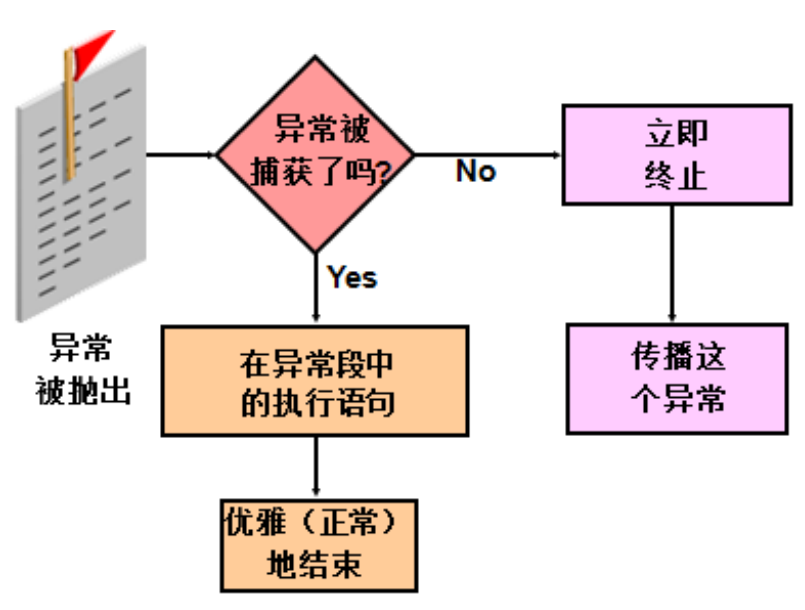
\includegraphics[width=0.7\textwidth]{picture/异常处理方式.png}
    \captionsetup{hypcap=false}
    \captionof{figure}{异常处理方式示意图}
    \label{fig:异常处理方式}
  \end{minipage}
\end{center}
\subsection{捕获异常}
在PL/SQL程序中包含了一个{\bfseries\kaishu 异常段(EXCEPTION section)}以捕获异常。如果异常在这个程序的执行段中被抛出,那么处理就自动跳转到这个程序的异常段中的相应异常处理程序。如果异常处理程序成功地处理了这个异常,那么这个异常就不会传播到包含它的程序段,也不会传播到调用环境,而这个PL/SQL程序块成功地结束。

语法:
\begin{plsql}[caption=捕获异常语法]
EXCEPTION
  -- 处理指定异常的代码
  WHEN 异常1 [或 异常2 …] THEN
    语句1;
    语句2;
    …
  [WHEN 异常1 [或 异常2 …] THEN
    语句1;
    语句2;
  …]
  [WHEN 异常1 [或 异常2 …] THEN
    语句1;
    语句2;
  …]
  -- 处理其他异常的代码
  [WHEN OTHERS THEN
    语句1;
    语句2;
  …]
\end{plsql}

\begin{description}
  \item[异常(exception)] 一 个 预 定 义 异 常 的 标 准 名 ( 如  TOO\_MANY\_ROWS)或在声明段中用户定义的异常名。
  \item[语句 (statement)] 一个或多个PL/SQL或SQL语句。
  \item[OTHERS] 一个可选的异常处理子句,该子句捕获任何没有显式处理的异常(就是在之前的所有WHEN子句都没有捕获的异常)
\end{description}

可以在一个异常段中包含任意多个异常处理程序(实际上就是任意多个WHEN子句)以处理说明的异常。然而, 对应一个单一的异常不能有多个处理程序;异常处理段只捕获那些声明了的异常,而任何其他的异常都不捕获,除非使用了OTHERS异常处理程序。

\begin{plsql}[caption=捕获异常示例代码]
BEGIN
  -- 主要执行部分
EXCEPTION
  WHEN ZERO_DIVIDE THEN
  -- 处理除零异常的代码
  WHEN OTHERS THEN
  -- 处理其他异常的代码
END;
\end{plsql}

\subsection{传播异常}
如果一个异常在程序的执行段被抛出并且没有对应的异常处理程序,那么{\bfseries\kaishu 这个PL/SQL程序块以失败而终止},并且这个异常被传播到包含它的程序块或调用环境,调用环境可以是任何应用程序。

\subsubsection{使用RAISE传播异常}
\begin{plsql}[caption=RAISE传播异常示例代码]
BEGIN
  -- 主要执行部分
EXCEPTION
  WHEN ZERO_DIVIDE THEN
  -- 处理除零异常的代码
  RAISE;    -- 在捕获的异常块中重新引发异常
  WHEN OTHERS THEN
  -- 处理其他异常的代码
  RAISE;    -- 在捕获的异常块中重新引发异常
END;
\end{plsql}
\subsubsection{使用RAISE\_APPLICATION\_ERROR传播异常}
RAISE\_APPLICATION\_ERROR是一个Oracle提供的过程,允许抛出一个错误号和消息,这个错误号的范围必须在-20000到-20999之间,以避免与 Oracle 内部错误码冲突。这允许你传播一个带有自定义消息的异常,这在封装异常信息和创建更具描述性的错误信息时非常有用。
\begin{plsql}[caption=RAISE\_APPLICATION\_ERROR传播异常示例代码]
EXCEPTION
  WHEN my_exception THEN
  RAISE_APPLICATION_ERROR(-20001, '自定义错误信息');
\end{plsql}
\section{异常类型}
在PL/SQL程序中可以使用的异常共有如下三种类型:
\begin{enumerate}
  \item 预定义的Oracle服务器错误(异常)。
  \item 非预定义的Oracle服务器错误(异常)。
  \item 用户定义的错误(异常)。
\end{enumerate}
\subsection{处理预定义的Oracle服务器错误}

\begin{plsql}[caption=处理预定义的Oracle服务器错误示例]
BEGIN
  -- 主要执行部分
EXCEPTION
  WHEN ZERO_DIVIDE THEN
  -- 处理除零异常的代码
  WHEN OTHERS THEN
  -- 处理其他异常的代码
END;
\end{plsql}
常见预定义异常:
\begin{center}
  \begin{minipage}{\textwidth}
    \center
    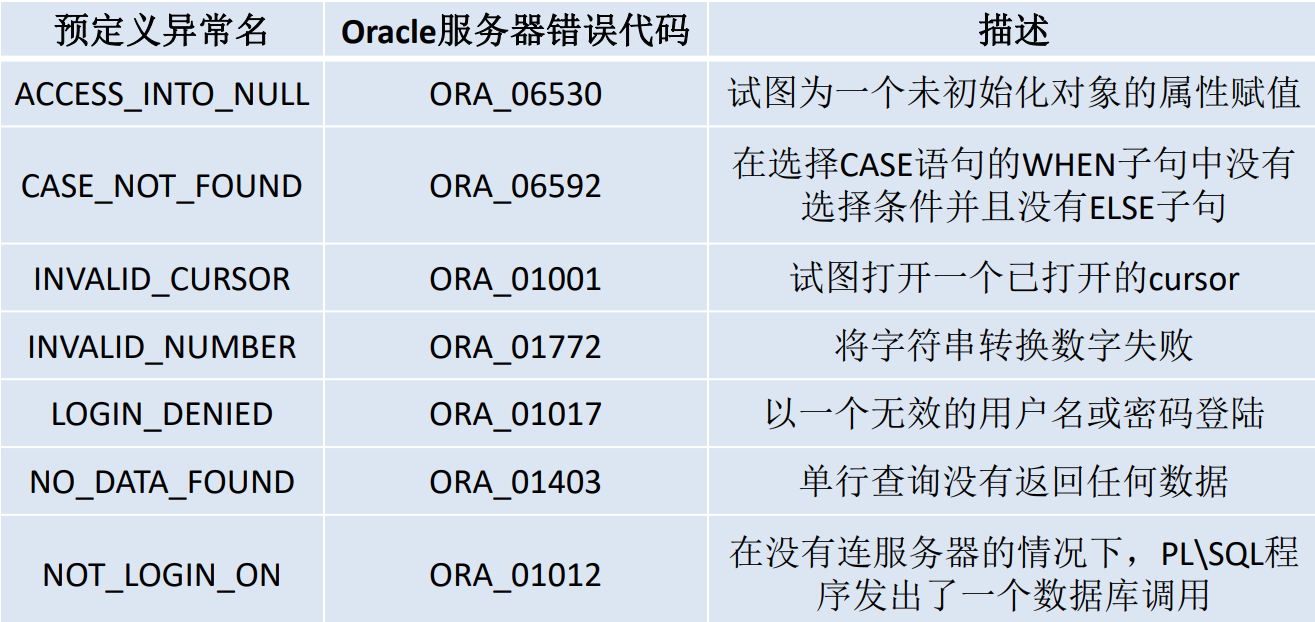
\includegraphics[width=1\textwidth]{picture/常见预定义异常.png}
    \captionsetup{hypcap=false}
    \captionof{figure}{常见预定义异常表}
    \label{fig:常见预定义异常}
  \end{minipage}
\end{center}

\subsection{处理非预定义的Oracle服务器错误}

非预定义的异常与预定义的异常非常相似,只是它们没有被定义为Oracle服务器中的PL/SQL异常而已,它们是标准的Oracle错误。
需使用{\bfseries\kaishu PRAGMA\ EXCEPTION\_INIT}将一个异常和一个 Oracle 错误代码关联起来,以便在捕获该异常时能够获取详细的错误信息。

PRAGMA(也被称为伪指令“pesudoinstructions”)是关键字,它表示这个语句是一个编译指令,而当PL/SQL程序块执行时不会被处理。PRAGMA关键字指示PL/SQL编译器将这个程序块中出现的所有该异常名解释成相关的Oracle服务器错误代码。

\begin{plsql}[caption=处理非预定义的Oracle服务器错误示例]
DECLARE
  no_permission_exception EXCEPTION;
  PRAGMA EXCEPTION_INIT(no_permission_exception, -942); 
BEGIN
  FOR emp_rec IN (SELECT * FROM employees) LOOP
    DBMS_OUTPUT.PUT_LINE('Employee ID: ' || emp_rec.employee_id);
  END LOOP;
EXCEPTION
  WHEN no_permission_exception THEN -- 处理没有权限的异常
    DBMS_OUTPUT.PUT_LINE('没有足够的权限访问 employees 表。');
  WHEN OTHERS THEN -- 处理其他异常的代码
  DBMS_OUTPUT.PUT_LINE('发生其他异常。');
END;
\end{plsql}

\subsection{处理用户定义的错误}
需使用{\bfseries\kaishu RAISE my\_exception;}显式抛出自定义异常。

声明和捕获用户定义的异常步骤:
\begin{enumerate}
  \item 在一个PL/SQL程序块的声明段中声明一个用户定义的异常。
  \item 使用RAISE语句显式地抛出这个异常。
  \item 在EXCEPTION段处理这个异常。
\end{enumerate}

\begin{plsql}[caption=处理用户定义的错误示例1]
DECLARE
  my_custom_exception EXCEPTION;
BEGIN
  -- 主要执行部分
  IF some_condition THEN -- 在某个条件下显式抛出自定义异常
    RAISE my_custom_exception;
  END IF;
EXCEPTION
  WHEN my_custom_exception THEN -- 处理自定义异常的代码
  WHEN OTHERS THEN -- 处理其他异常的代码
END;
\end{plsql}

\begin{plsql}[caption=处理用户定义的错误示例2]
DECLARE
  -- 步骤 1: 在声明段中声明用户定义的异常
  department_not_found EXCEPTION;
  PRAGMA EXCEPTION_INIT(department_not_found, -20001);
  v_department_id NUMBER := &p_department_id; -- 用户输入的部门号
BEGIN
  -- 步骤 2: 检查部门是否存在,如果不存在则抛出用户定义的异常
  IF NOT EXISTS (SELECT 1 FROM departments WHERE department_id = v_department_id) THEN
    RAISE department_not_found;
  END IF;
  -- 在这里执行其他操作,因为部门存在
EXCEPTION
  -- 步骤 3: 在 EXCEPTION 段中捕获用户定义的异常并处理
  WHEN department_not_found THEN
    DBMS_OUTPUT.PUT_LINE('用户定义的异常:部门不存在。');
END;
\end{plsql}

\section{捕获异常实例}
\begin{plsql}[caption=一个捕获异常的实例]
DECLARE
  -- 自定义异常
  emp_not_found EXCEPTION;
  invalid_dept EXCEPTION;
  application_error EXCEPTION;
  -- 假设的员工编号和部门编号
  v_empno emp.empno%TYPE := 1001;
  v_deptno dept.deptno%TYPE := 10;
  -- 用于检查的变量
  v_count NUMBER;
BEGIN
  -- 检查员工是否存在
  SELECT COUNT(*)
  INTO v_count
  FROM emp
  WHERE empno = v_empno;
  IF v_count = 0 THEN
    RAISE emp_not_found;
  END IF;
  -- 检查部门是否有效
  SELECT COUNT(*)
  INTO v_count
  FROM dept
  WHERE deptno = v_deptno;
  IF v_count = 0 THEN
    RAISE invalid_dept;
  END IF;
  - 执行更新操作
  UPDATE emp
  SET deptno = v_deptno
  WHERE empno = v_empno;
  -- 提交事务
  COMMIT;
EXCEPTION
  WHEN emp_not_found THEN
    DBMS_OUTPUT.PUT_LINE('员工编号 ' || v_empno || ' 不存在。');
    ROLLBACK;
  WHEN invalid_dept THEN
    DBMS_OUTPUT.PUT_LINE('部门编号 ' || v_deptno || ' 无效。');
    ROLLBACK;
  WHEN OTHERS THEN  -- 捕获其他所有未处理的异常
    DBMS_OUTPUT.PUT_LINE('发生未知错误: ' || SQLERRM);
    ROLLBACK;
    RAISE; -- 重新抛出异常
END;
/
\end{plsql}

\section{SQLCODE和SQLERRM}
PL/SQL提供了两个函数,当一个异常发生时,可以通过使用这两个函数来标识相关的错误代码信息。这二个函数就是SQLCODE和SQLERRM,{\bfseries\kaishu SQLCODE函数为内部异常返回一个Oracle错误号码,而SQLERRM函数则返回与这个错误号码相关的信息}。

使用示例:
\begin{plsql}[caption=SQLCODE和SQLERRM示例代码]
DECLARE
  my_exception EXCEPTION;
BEGIN
  -- 一个可能引发异常的 SQL 语句
  SELECT 1 / 0 INTO my_variable FROM dual;
EXCEPTION
  WHEN OTHERS THEN
    -- 获取异常的错误代码
    DBMS_OUTPUT.PUT_LINE('SQLCODE: ' || SQLCODE);
    -- 获取异常的详细错误信息
    DBMS_OUTPUT.PUT_LINE('SQLERRM: ' || SQLERRM);
END;
\end{plsql}

\section{处理异常建议}
Oracle推荐在开发捕获异常的PL/SQL程序代码时应该注意如下事项:
\begin{enumerate}
  \item 以关键字EXCEPTION开始异常处理程序的程序段。
  \item 在异常段中可以定义若干个异常处理程序(子句),每一个都有自己的一组操作。
  \item 当一个异常发生时,PL/SQL在离开这个异常段之前只执行一个异常处理子句。
  \item 将OTHERS子句放在所有其他异常处理子句之后。
  \item 在一个异常段中只能有一个OTHER子句。
  \item 异常不能出现在赋值语句中,也不能出现在SQL语句中。
\end{enumerate}

使用SQLCODE和SQLERRM的建议:
\begin{plsql}[caption=记录异常(需先建立错误记录表)]
EXCEPTION
  WHEN OTHERS THEN
    ROLLBACK;
    v_error_code := SQLCODE;
    v_error_message := SQLERRM;
    INSERT INTO errors (user_name, error_date, error_code, error_message)
    VALUES (USER, SYSDATE, v_error_code, v_error_message);
    COMMIT;
\end{plsql}
\begin{enumerate}
  \item {\bfseries\kaishu 监测频繁的错误:}通过查询errors表并计算每个error\_code的出现次数,可以识别出频繁出  现的错误。这通常通过一个简单的SELECT error\_code, COUNT(*) FROM errors GROUP BY error\_code查询来实现。
  \item {\bfseries\kaishu 为常见错误定义异常:}对于每个频繁出现的错误代码,可以声明一个特定的异常,并使用 PRAGMA EXCEPTION\_INIT将其与错误代码关联。这样就可以在PL/SQL程序中直接引用这些异常。
  \item {\bfseries\kaishu 增加异常处理逻辑:}在PL/SQL块的异常部分,可以为每个常见的错误代码增加一个WHEN子句。在这个子句中,可以编写特定的处理逻辑,如记录额外的信息、发送通知或采取其他纠正措施。
  \item {\bfseries\kaishu 清理errors表:}在处理完一个常见错误后,可以从errors表中删除与该错误代码关联的所有记录。这样做可以确保rrors表中只保留那些偶尔发生的、不常见的错误。
  \item {\bfseries\kaishu 代码维护和调试:}使用SQLCODE和SQLERRM可以在调试阶段帮助开发者理解错误的原因。一旦调试完毕,这些语句可以被注释掉或删除,以避免生产环境中不必要的性能开销。
\end{enumerate}

\chapter{过程}
在PL/SQL程序设计中,{\bfseries\kaishu 子程序(也称为过程或函数)}是模块化程序设计的基础。要使子程序更灵活,重要的一点是可以改变所操作的数据(即可以通过计算,也可以通过使用输入参数传递给一个子程序),而子程序计算的结果可以通过输出(OUT)参数返回给子程序的调用者。{\bfseries\kaishu 子程序的目的是通过将代码组织成可重用的单元来提高代码的可维护性和可读性。}

\begin{plsql}[caption=子程序示例]
--定义过程
CREATE OR REPLACE PROCEDURE CalculateSquare(
  p_number IN NUMBER,
  p_result OUT NUMBER
) AS
BEGIN
  -- 计算平方
  p_result := p_number * p_number;
END;

--调用过程
DECLARE
  v_input NUMBER := 5;
v _output NUMBER;
BEGIN
  CalculateSquare(v_input, v_output);
  DBMS_OUTPUT.PUT_LINE('Square of ' || v_input || ' is ' || v_output);
END;
\end{plsql}
\section{模块化与分层}
利用子程序进行{\bfseries\kaishu 模块化}程序设计的基本原则是:尽可能地创建较小的、灵活的、可重用的代码段以方便程序的管理和维护。
灵活性是通过使用带有参数的子程序而获得的,而正是这种灵活性又通过使用不同的输入值使得相同的程序代码能够重用。

模块化{\bfseries\kaishu 现存的程序代码}的步骤:
\begin{enumerate}
  \item 定位和标识重复的程序代码序列。
  \item 将这些重复的程序代码移到一个PL/SQL子程序中。
  \item 将原来的重复程序代码以新的PL/SQL子程序调用代替。
\end{enumerate}

模块化的优势:
\begin{enumerate}
  \item {\bfseries\kaishu 语法分析重用:}优化器能够有效地重复利用经过解析的SQL语句,更好地利用服务器资源。
  \item 可维护性:将业务逻辑分解为独立的模块,使得对系统进行更新、修复或新增功能变得更加简单。
  \item 可读性:代码结构更加清晰。
  \item 性能优化:通过将复杂的业务逻辑分解为独立的模块,优化器可以更精确地评估每个模块的性能,并采取相应的优化措施。
  \item 减少代码冗余:将通用功能抽象为可重用的模块,可以避免在不同部分中重复编写相似的代码。
\end{enumerate}

分层设计思路:
\begin{enumerate}
  \item 数据访问层:使用SQL语句访问数据库子程序。
  \begin{enumerate}
    \item 使用 SQL 语句访问数据库。
    \item 封装数据库细节。
    \item 提供数据访问接口。
  \end{enumerate}
  \item 业务逻辑层:实现业务处理规则的子程序,这些子程序可以调用也可以不调用数据访问层的子程序。
  \begin{enumerate}
    \item 实现业务处理规则。
    \item 调用数据访问层。
    \item 与用户界面交互。
  \end{enumerate}
\end{enumerate}

与模块化有关的组件:
\begin{itemize}
  \item 匿名程序块。
  \item 子程序(过程和函数)。
  \item 软件包。
  \item 数据库触发器。
\end{itemize}

\section{子程序}
子程序是基于标准的PL/SQL结构的,其实就是一个命名的PL/SQL程序块,它可以接收参数和在调用环境中被调用。子程序包括一个声明段、一个执行段和一个可选的异常处理段。子程序可以被编译或存储在数据库中以提高模块化、可扩展性和重用性,以及方便维护。

一个PL/SQL子程序就是一个命名的、可以使用一组参数调用的PL/SQL程序块。可以在一个PL/SQL程序块中也可以在另一个子程序中声明和定义子程序。 

\begin{plsql}[caption=子程序语法模版]
--子程序说明部分
<header>

IS | AS
--子程序体
  Declaration 部分
BEGIN
  可执行部分
EXCEPTION (optional)
  异常部分
END;
\end{plsql}

PL/SQL有两种类型的子程序,即过程和函数。{\bfseries\kaishu 通常,使用过程来执行一个操作,而使用一个函数计算并返回一个值。}过程和函数具有相同的结构,它们唯一的区别是\textbf{函数有一个额外的项——RETURN子句或RETURN语句}。

\begin{plsql}[caption=过程示例]
CREATE OR REPLACE PROCEDURE my_procedure(p_parameter IN VARCHAR2) 
  IS
BEGIN
  -- Procedure code here
  DBMS_OUTPUT.PUT_LINE('Parameter received: ' || p_parameter);
END my_procedure;
\end{plsql}

\begin{plsql}[caption=函数示例]
CREATE OR REPLACE FUNCTION calculate_area(radius NUMBER) RETURN NUMBER 
  IS
  v_area NUMBER;
BEGIN
  v_area := 3.14 * radius * radius;
  RETURN v_area;
END calculate_area;
\end{plsql}

匿名程序块与子程序之间的差别:
\begin{enumerate}
  \item 子程序只编译一次;匿名程序块在执行时编译。(如果想重用一个匿名块,就必须重新运行创建这个匿名块的脚本,这会造成重新编译和执行)
  \item 子程序可以存储在数据库中;匿名程序块不可以。
  \item 子程序可以被其他程序调用;匿名程序块不可以。
  \item 子程序的函数必须有返回值;匿名程序块不能带返回值。
  \item 子程序可以有参数;匿名程序块不能有参数。
\end{enumerate}

\section{过程}

\subsection{过程语法}
过程是指可以接收参数并命名的PL/SQL程序块,过程是子程序的一种类型,通常使用它来执行一个动作。过程包括\textbf{过程头、声明段、执行段和可选的异常处理段}。在另外的PL/SQL程序块的执行段中通过使用过程名调用这个过程。

在PL/SQL中,可以使用SQL的{\bfseries\kaishu CREATE[OR REPLACE]PROCEDURE}语句创建存储在数据库中的独立过程。一个过程与一个微型的程序类似——执行一个特定的操作。在创建过程语句中,要说明过程名、过程的参数、过程的本地变量和包括过程代码和处理代码的BEGIN-END所包括的程序块。

\begin{plsql}[caption=创建过程的语法]
CREATE [OR REPLACE] PROCEDURE 过程名
  [(参数1 [参数模式] 数据类型1,参数2 [参数模式] 数据类型2, …)]
IS|AS
  [本地变量的声明; …]
BEGIN
  -- 执行的操作;
END [过程名];
\end{plsql}

参数可以被看作本地变量。在一个PL/SQL存储过程的定义中,参数和本地变量在合适的作用域内都是可以被引用的。

\begin{plsql}[caption=创建过程示例代码]
CREATE OR REPLACE PROCEDURE ExampleProcedure (
 p_input_param IN VARCHAR2,
 p_output_param OUT NUMBER
) IS
  -- 这是一个本地变量,只在当前存储过程中可见
  v_local_variable NUMBER := 0;
BEGIN
  -- 使用输入参数
  DBMS_OUTPUT.PUT_LINE('Input parameter: ' || p_input_param);
  -- 修改本地变量的值
  v_local_variable := 42;
  -- 使用输出参数
  p_output_param := v_local_variable;
  -- 在这里可以引用输入参数、输出参数和本地变量
END ExampleProcedure;
\end{plsql}

\subsection{过程参数数据类型}
可以使用如下方法制定参数的数据类型:
\begin{enumerate}
  \item {\bfseries\kaishu 显式数据类型:}如p\_param1 VARCHAR2(50)。
  \item {\bfseries\kaishu \%TYPE定义:}如p\_param2 employees.salary\%TYPE。
  \item {\bfseries\kaishu \%ROWTYPE定义:}如p\_param2 employees\%ROWTYPE。
\end{enumerate}

\subsection{过程参数的参数模式}

参数被用来在调用环境和过程之间进行数据的传递。参数是在子程序(过程)的头中声明的,即在过程名之后和本地变量声明段之前,调用环境和过程之间进行参数传递的操作。

\begin{enumerate}
  \item {\bfseries\kaishu IN参数:}从调用环境传递一个常数值给过程,可赋予默认值。(默认)
  \item {\bfseries\kaishu OUT参数:}从过程传递一个值给调用环境,实参必须为变量,不可赋予默认值。
  \item {\bfseries\kaishu IN OUT参数:}从调用环境传递一个值给过程,并且使用相同的参数名从过程返回给调用环境一个可能不同的值,实参必须为变量,不可赋予默认值。
\end{enumerate}

可以把参数看成本地变量的一种特殊形式;当子程序被调用时,参数的输入值由调用环境初始化,并且当子程序将控制返回给调用者时,参数的输出值被返回给调用环境。

\begin{plsql}[caption=IN参数模式实例]
--为某一个员工提升工资的过程
CREATE OR REPLACE PROCEDURE raise_salary(p_empno IN emp_pl.empno%TYPE,p_rate IN NUMBER)
IS
BEGIN
  UPDATE emp_pl
  SET sal = sal * (1 + p_rate * 0.01)
  WHERE empno = p_empno;
END raise_salary;
/
\end{plsql}

\begin{plsql}[caption=OUT参数模式实例]
--输出指定员工信息
CREATE OR REPLACE PROCEDURE get_employee
  (p_empno IN emp_pl.empno%TYPE,
  p_name OUT emp.ename%TYPE,
  p_salary OUT emp.sal%TYPE,
  p_job OUT emp.job%TYPE)
IS
BEGIN
  SELECT ename, sal, job
  INTO p_name, p_salary, p_job
  FROM emp
  WHERE empno = p_empno;
END;
/
\end{plsql}

\begin{plsql}[caption=IN OUT参数模式实例]
--将输入的电话号码转换为标准的容易阅读格式
CREATE OR REPLACE PROCEDURE standard_phone
  (p_phone_no IN OUT VARCHAR2) 
IS
BEGIN
  p_phone_no := '(' || SUBSTR(p_phone_no,1,3) ||')' || SUBSTR(p_phone_no,4,3) ||'-' || SUBSTR(p_phone_no,7);
END standard_phone;
\end{plsql}

\subsection{绑定变量获得过程的OUT输出}
步骤:
\begin{enumerate}
  \item 声明过程变量:{\bfseries\kaishu VARIABLE myvar NUMBER}。
  \item (可选:如果是IN OUT参数需要为这个数字变量赋初值:{\bfseries\kaishu EXEC :myvar := 10}。)
  \item 以绑定变量为参数执行过程:{\bfseries\kaishu EXEC my\_procedure(:myvar)}。
  \item 使用PRINT命令打印绑定变量:{\bfseries\kaishu PRINT myvar}。
\end{enumerate}

\subsection{在过程中处理异常}
在过程中处理异常的方式与在一般程序块中处理异常的方法完全相同:
当在一个调用过程中抛出一个异常时,程序的控制立刻跳转到这个程序块的异常段。如果这个异常段提供了一个处理所抛出异常的异常处理程序,那么这个异常被认定处理了。

PL/SQL将执行如下代码流程:
\begin{enumerate}
  \item 这个异常被抛出。
  \item 控制转移到匹配的异常处理程序。
  \item 执行异常处理程序的代码块。
  \item 异常处理程序执行完成后,程序块执行结束。
\end{enumerate}

如果一个DML操作是在异常之前在异常所在的过程中执行的,那么这个DML操作被回滚。

\begin{plsql}[caption=过程异常处理示例代码]
 CREATE OR REPLACE PROCEDURE add_depte
  (p_name IN dept_pl.dname%TYPE DEFAULT '服务',
  p_loc IN dept_pl.loc%TYPE DEFAULT '狼山镇')
IS
BEGIN
  INSERT INTO dept_pl
  VALUES (deptid_sequence.NEXTVAL, p_name, p_loc);
  DBMS_OUTPUT.PUT_LINE('添加部门:'||p_name);
EXCEPTION
  WHEN OTHERS THEN
    DBMS_OUTPUT.PUT_LINE('错误:添加部门:'||p_name);
END add_depte;
/
\end{plsql}

\subsection{在过程中抛出异常}
当被调用过程的异常段没有提供所抛出异常的处理程序时,PL/SQL程序代码流程如下:
\begin{enumerate}
  \item 抛出异常。
  \item 程序块结束,因为不存在异常处理程序,在该过程中所执行的任何DML操作全部被回滚。
  \item 异常传播到调用过程的异常段,即控制返回到调用块的异常段。
\end{enumerate}

如果一个异常没有被处理,那么{\bfseries\kaishu 在调用过程和被调用过程中的所有DML语句连同对任何绑定变量的更改一起全部被回滚}。但是在调用抛出异常过程之前所执行的DML语句并不受影响。

\section{实参的传递方式}
PL/SQL提供了三种不同的参数传递表示法,分别{\bfseries\kaishu 按位置(position)}、{\bfseries\kaishu 按名字(Named)}和{\bfseries\kaishu 组合(Combination)表示法}。

\begin{description}
  \item[按位置] 以所声明的形参相同的顺序列出实参。
  \item[按名字] 以任意顺序列出实参和与之相关的对应形参,但要是使用关联操作符将每一个实参与对应的形参用名关联起来。
  \item[组合] 部分实参按位置,部分实参按名称。
\end{description}

在开发一个子程序时可以将几乎所有的可能情况考虑进去,这样可能需要很多形参。但是在使用时用户并不需要了解全部参数,一个用户只需要理解他所需要的参数即可。
\begin{plsql}[caption=按位置传递示例]
CREATE OR REPLACE PROCEDURE example_proc
  (p_name IN VARCHAR2, p_age IN NUMBER) 
IS
BEGIN
  -- procedure body
END example_proc;

-- 调用过程
EXEC example_proc('John', 30);
\end{plsql}

\begin{plsql}[caption=按参数名传递示例]
CREATE OR REPLACE PROCEDURE example_proc
  (p_name IN VARCHAR2, p_age IN NUMBER) 
IS
BEGIN
  -- procedure body
END example_proc;

-- 调用过程,通过参数名传递
EXEC example_proc(p_age => 30, p_name => 'John');
\end{plsql}

\begin{plsql}[caption=组合传递示例]
CREATE OR REPLACE PROCEDURE example_proc
  (p_name IN VARCHAR2, p_age IN NUMBER) IS
BEGIN
  -- procedure body
END example_proc;
  
-- 调用过程,混合使用按位置和按名字传递
EXEC example_proc('John', p_age => 30);
\end{plsql}

\chapter{游标}
在PL/SQL中,游标(CURSOR)是一种数据库查询的控制结构,它用于存储从SQL语句如SELECT查询返回的结果集。游标使得开发者能够在PL/SQL程序中逐行处理查询结果。

游标用途:
\begin{enumerate}
  \item 逐行处理数据。
  \item 复杂逻辑的实现。
  \item 锁定行。
  \item 资源优化。
\end{enumerate}

\section{游标类型}
\begin{enumerate}
  \item 显式游标:开发者需要显式声明、打开、获取数据、关闭。这给了开发者更多的控制,但也需要更多的代码。
  \item 隐式游标:Oracle 为 每 个 SQL DML 语 句 ( 如 INSERT, UPDATE,  DELETE, SELECT INTO)提供的自动游标。它们不需要  显式声明和管理,但控制较少。
\end{enumerate}
\section{游标的操作过程}
\begin{enumerate}
  \item 声明:CURSOR my\_cursor IS SELECT column1, column2 FROM my\_table WHERE condition;  
  \item 打开:OPEN my\_cursor;
  \item 提取:FETCH my\_cursor INTO variable1, variable2;
  \item 关闭:CLOSE my\_cursor;
\end{enumerate}

\section{游标逐行处理数据示例}
\begin{plsql}[caption=游标逐行处理数据示例1]
-- 创建一个简单的表
CREATE TABLE employee (
  emp_id NUMBER PRIMARY KEY,
  emp_name VARCHAR2(50),
  emp_salary NUMBER
);

-- 插入一些示例数据
INSERT INTO employee VALUES (1, 'Alice', 50000);
INSERT INTO employee VALUES (2, 'Bob', 60000);
INSERT INTO employee VALUES (3, 'Charlie', 70000);

-- 创建一个存储过程,使用游标逐行处理数据
CREATE OR REPLACE PROCEDURE display_employee_data 
IS
  -- 定义游标
  CURSOR emp_cursor IS
    SELECT emp_id, emp_name, emp_salary FROM employee;
  
  -- 定义变量来存储检索到的列值
  v_emp_id employee.emp_id%TYPE;
  v_emp_name employee.emp_name%TYPE;
  v_emp_salary employee.emp_salary%TYPE;
BEGIN
  -- 打开游标
  OPEN emp_cursor;
  -- 逐行处理数据
  LOOP
    -- 从游标中检索数据
    FETCH emp_cursor INTO v_emp_id, v_emp_name, v_emp_salary;
    -- 判断是否还有数据
    EXIT WHEN emp_cursor%NOTFOUND;
    -- 处理当前行数据,这里简单地显示在输出
    DBMS_OUTPUT.PUT_LINE('Employee ID: ' || v_emp_id || ', Name: ' || v_emp_name || ', Salary: ' || v_emp_salary);
  END LOOP;

  -- 关闭游标
  CLOSE emp_cursor;
END;
/

-- 执行存储过程以显示数据
SET SERVEROUTPUT ON;
EXEC display_employee_data;
\end{plsql}

使用FOR循环简化:FOR循环是一种简化的循环结构,它允许在循环声明中直接指定一个游标,并在循环体内自动处理每一行,无需显式地使用OPEN、FETCH和CLOSE语句。
\begin{plsql}[caption=游标逐行处理数据示例2]
-- 创建一个简单的表
CREATE TABLE employee (
  emp_id NUMBER PRIMARY KEY,
  emp_name VARCHAR2(50),
  emp_salary NUMBER
);

-- 插入一些示例数据
INSERT INTO employee VALUES (1, 'Alice', 50000);
INSERT INTO employee VALUES (2, 'Bob', 60000);
INSERT INTO employee VALUES (3, 'Charlie', 70000);

-- 创建一个存储过程,使用FOR循环处理数据
CREATE OR REPLACE PROCEDURE display_employee_data 
IS
BEGIN
  -- 使用FOR循环声明游标和直接处理每一行
  FOR emp_rec IN (SELECT emp_id, emp_name, emp_salary FROM employee) LOOP
    -- 在循环体内直接访问每一行的字段
    DBMS_OUTPUT.PUT_LINE('Employee ID: ' || emp_rec.emp_id || ', Name: ' || emp_rec.emp_name || ', Salary: ' || emp_rec.emp_salary);
  END LOOP;
END;
/

-- 执行存储过程以显示数据
SET SERVEROUTPUT ON;
EXEC display_employee_data;
\end{plsql}

% 文章结束
\end{document}